\documentclass[10pt,twocolumn]{article}

\usepackage[margin=0.75in,columnsep=0.25in]{geometry}
\usepackage[T1]{fontenc}
\usepackage{lmodern}
\usepackage{textcomp}
\usepackage{microtype}
\usepackage{booktabs}
\usepackage{graphicx}
\usepackage{xcolor}
\usepackage{pgfplots}
\pgfplotsset{compat=1.18}
\usepackage[numbers,sort&compress]{natbib}
\usepackage[hidelinks]{hyperref}
\usepackage{xurl}

% Every measured number comes from paper/data through paper/gen.py. Write
% \data{key}; an unknown key stops the build. paper/check_numbers.py fails on
% digits typed into these sources.
\makeatletter
\newcommand{\data}[1]{%
  \ifcsname pqd@#1\endcsname\csname pqd@#1\endcsname
  \else\errmessage{paper: no value for data key '#1' (run python3 paper/gen.py)}\fi}
\makeatother
% Generated by paper/gen.py from paper/data. Do not edit.
% \data{key} expands to the value; an unknown key stops the build.
\expandafter\def\csname pqd@riskabl-confidence-reversed\endcsname{0.8\%}
\expandafter\def\csname pqd@riskabl-confidence-tau\endcsname{0.992}
\expandafter\def\csname pqd@riskabl-confidence-tied\endcsname{1.2\%}
\expandafter\def\csname pqd@riskabl-confidence-top\endcsname{19}
\expandafter\def\csname pqd@riskabl-confidence-top-share\endcsname{26\%}
\expandafter\def\csname pqd@riskabl-exposure-reversed\endcsname{6.8\%}
\expandafter\def\csname pqd@riskabl-exposure-tau\endcsname{0.786}
\expandafter\def\csname pqd@riskabl-exposure-tied\endcsname{9.3\%}
\expandafter\def\csname pqd@riskabl-exposure-top\endcsname{45}
\expandafter\def\csname pqd@riskabl-exposure-top-share\endcsname{62\%}
\expandafter\def\csname pqd@riskabl-findings\endcsname{13,082}
\expandafter\def\csname pqd@riskabl-pairs\endcsname{4,529,502}
\expandafter\def\csname pqd@riskabl-projects\endcsname{72}
\expandafter\def\csname pqd@riskabl-quantum-status-reversed\endcsname{16.4\%}
\expandafter\def\csname pqd@riskabl-quantum-status-tau\endcsname{0.593}
\expandafter\def\csname pqd@riskabl-quantum-status-tied\endcsname{4.4\%}
\expandafter\def\csname pqd@riskabl-quantum-status-top\endcsname{34}
\expandafter\def\csname pqd@riskabl-quantum-status-top-share\endcsname{47\%}
\expandafter\def\csname pqd@riskabl-revision\endcsname{v0.12.0-8-gbd66d35}
\expandafter\def\csname pqd@riskabl-secrecy-lifetime-reversed\endcsname{12.1\%}
\expandafter\def\csname pqd@riskabl-secrecy-lifetime-tau\endcsname{0.897}
\expandafter\def\csname pqd@riskabl-secrecy-lifetime-tied\endcsname{1.4\%}
\expandafter\def\csname pqd@riskabl-secrecy-lifetime-top\endcsname{28}
\expandafter\def\csname pqd@riskabl-secrecy-lifetime-top-share\endcsname{39\%}
\expandafter\def\csname pqd@rqfour-ch-classical\endcsname{245}
\expandafter\def\csname pqd@rqfour-ch-default\endcsname{1,477}
\expandafter\def\csname pqd@rqfour-ch-extra\endcsname{1,184}
\expandafter\def\csname pqd@rqfour-ch-hybrid\endcsname{1,429}
\expandafter\def\csname pqd@rqfour-ch-ratio\endcsname{5.8$\times$}
\expandafter\def\csname pqd@rqfour-ch-segments\endcsname{1}
\expandafter\def\csname pqd@rqfour-circl\endcsname{v1.6.5}
\expandafter\def\csname pqd@rqfour-client-bytes-classical\endcsname{309}
\expandafter\def\csname pqd@rqfour-client-bytes-hybrid\endcsname{1,493}
\expandafter\def\csname pqd@rqfour-cores\endcsname{8}
\expandafter\def\csname pqd@rqfour-cpu\endcsname{Apple M2}
\expandafter\def\csname pqd@rqfour-date\endcsname{2026-11-08}
\expandafter\def\csname pqd@rqfour-docker-failures\endcsname{0}
\expandafter\def\csname pqd@rqfour-docker-handshakes\endcsname{4,500}
\expandafter\def\csname pqd@rqfour-docker-kernel\endcsname{Linux 6.12.76-linuxkit}
\expandafter\def\csname pqd@rqfour-docker-mem-gb\endcsname{3.8}
\expandafter\def\csname pqd@rqfour-ecdh-p256-go-stdlib-decap-p50\endcsname{40.8\,\textmu s}
\expandafter\def\csname pqd@rqfour-ecdh-p256-go-stdlib-decap-p99\endcsname{52.0\,\textmu s}
\expandafter\def\csname pqd@rqfour-ecdh-p256-go-stdlib-encap-p50\endcsname{52.0\,\textmu s}
\expandafter\def\csname pqd@rqfour-ecdh-p256-go-stdlib-encap-p99\endcsname{66.3\,\textmu s}
\expandafter\def\csname pqd@rqfour-ecdh-p256-go-stdlib-keygen-p50\endcsname{11.1\,\textmu s}
\expandafter\def\csname pqd@rqfour-ecdh-p256-go-stdlib-keygen-p99\endcsname{19.5\,\textmu s}
\expandafter\def\csname pqd@rqfour-ecdsa-p256-go-stdlib-keygen-p50\endcsname{11.6\,\textmu s}
\expandafter\def\csname pqd@rqfour-ecdsa-p256-go-stdlib-keygen-p99\endcsname{23.7\,\textmu s}
\expandafter\def\csname pqd@rqfour-ecdsa-p256-go-stdlib-sign-p50\endcsname{21.8\,\textmu s}
\expandafter\def\csname pqd@rqfour-ecdsa-p256-go-stdlib-sign-p99\endcsname{30.5\,\textmu s}
\expandafter\def\csname pqd@rqfour-ecdsa-p256-go-stdlib-verify-p50\endcsname{54.8\,\textmu s}
\expandafter\def\csname pqd@rqfour-ecdsa-p256-go-stdlib-verify-p99\endcsname{72.9\,\textmu s}
\expandafter\def\csname pqd@rqfour-go\endcsname{1.26.3}
\expandafter\def\csname pqd@rqfour-handshake-bytes-extra\endcsname{2,272}
\expandafter\def\csname pqd@rqfour-handshake-bytes-ratio\endcsname{3.1$\times$}
\expandafter\def\csname pqd@rqfour-host-n\endcsname{1,000}
\expandafter\def\csname pqd@rqfour-host-p50-classical\endcsname{317\,\textmu s}
\expandafter\def\csname pqd@rqfour-host-p50-extra\endcsname{124\,\textmu s}
\expandafter\def\csname pqd@rqfour-host-p50-hybrid\endcsname{442\,\textmu s}
\expandafter\def\csname pqd@rqfour-hybrid-encap-vs-x25519\endcsname{1.5$\times$}
\expandafter\def\csname pqd@rqfour-hybrid-kex-extra\endcsname{111\,\textmu s}
\expandafter\def\csname pqd@rqfour-hybrid-kex-total\endcsname{251\,\textmu s}
\expandafter\def\csname pqd@rqfour-kernel\endcsname{Darwin 27.0.0}
\expandafter\def\csname pqd@rqfour-loopback-extra\endcsname{0.15\,ms}
\expandafter\def\csname pqd@rqfour-loopback-extra-rel\endcsname{48\%}
\expandafter\def\csname pqd@rqfour-loopback-mtu1500-extra\endcsname{0.15\,ms}
\expandafter\def\csname pqd@rqfour-loopback-mtu1500-extra-rel\endcsname{50\%}
\expandafter\def\csname pqd@rqfour-loopback-mtu1500-n\endcsname{200}
\expandafter\def\csname pqd@rqfour-loopback-mtu1500-p50-classical\endcsname{0.31\,ms}
\expandafter\def\csname pqd@rqfour-loopback-mtu1500-p50-default\endcsname{0.46\,ms}
\expandafter\def\csname pqd@rqfour-loopback-mtu1500-p50-hybrid\endcsname{0.46\,ms}
\expandafter\def\csname pqd@rqfour-loopback-mtu1500-p99-classical\endcsname{0.60\,ms}
\expandafter\def\csname pqd@rqfour-loopback-mtu1500-p99-hybrid\endcsname{0.97\,ms}
\expandafter\def\csname pqd@rqfour-loopback-n\endcsname{200}
\expandafter\def\csname pqd@rqfour-loopback-p50-classical\endcsname{0.31\,ms}
\expandafter\def\csname pqd@rqfour-loopback-p50-default\endcsname{0.45\,ms}
\expandafter\def\csname pqd@rqfour-loopback-p50-hybrid\endcsname{0.46\,ms}
\expandafter\def\csname pqd@rqfour-loopback-p99-classical\endcsname{0.98\,ms}
\expandafter\def\csname pqd@rqfour-loopback-p99-hybrid\endcsname{1.48\,ms}
\expandafter\def\csname pqd@rqfour-loss-pct\endcsname{1\%}
\expandafter\def\csname pqd@rqfour-loss-rtt\endcsname{40}
\expandafter\def\csname pqd@rqfour-mem-gb\endcsname{8}
\expandafter\def\csname pqd@rqfour-ml-dsa-44-circl-keygen-p50\endcsname{80.2\,\textmu s}
\expandafter\def\csname pqd@rqfour-ml-dsa-44-circl-keygen-p99\endcsname{219\,\textmu s}
\expandafter\def\csname pqd@rqfour-ml-dsa-44-circl-sign-p50\endcsname{147\,\textmu s}
\expandafter\def\csname pqd@rqfour-ml-dsa-44-circl-sign-p99\endcsname{959\,\textmu s}
\expandafter\def\csname pqd@rqfour-ml-dsa-44-circl-verify-p50\endcsname{73.3\,\textmu s}
\expandafter\def\csname pqd@rqfour-ml-dsa-44-circl-verify-p99\endcsname{120\,\textmu s}
\expandafter\def\csname pqd@rqfour-ml-dsa-65-circl-keygen-p50\endcsname{145\,\textmu s}
\expandafter\def\csname pqd@rqfour-ml-dsa-65-circl-keygen-p99\endcsname{281\,\textmu s}
\expandafter\def\csname pqd@rqfour-ml-dsa-65-circl-sign-p50\endcsname{238\,\textmu s}
\expandafter\def\csname pqd@rqfour-ml-dsa-65-circl-sign-p99\endcsname{1.25\,ms}
\expandafter\def\csname pqd@rqfour-ml-dsa-65-circl-verify-p50\endcsname{120\,\textmu s}
\expandafter\def\csname pqd@rqfour-ml-dsa-65-circl-verify-p99\endcsname{230\,\textmu s}
\expandafter\def\csname pqd@rqfour-ml-dsa-87-circl-keygen-p50\endcsname{216\,\textmu s}
\expandafter\def\csname pqd@rqfour-ml-dsa-87-circl-keygen-p99\endcsname{362\,\textmu s}
\expandafter\def\csname pqd@rqfour-ml-dsa-87-circl-sign-p50\endcsname{259\,\textmu s}
\expandafter\def\csname pqd@rqfour-ml-dsa-87-circl-sign-p99\endcsname{1.26\,ms}
\expandafter\def\csname pqd@rqfour-ml-dsa-87-circl-verify-p50\endcsname{199\,\textmu s}
\expandafter\def\csname pqd@rqfour-ml-dsa-87-circl-verify-p99\endcsname{334\,\textmu s}
\expandafter\def\csname pqd@rqfour-ml-kem-1024-circl-decap-p50\endcsname{38.2\,\textmu s}
\expandafter\def\csname pqd@rqfour-ml-kem-1024-circl-decap-p99\endcsname{43.5\,\textmu s}
\expandafter\def\csname pqd@rqfour-ml-kem-1024-circl-encap-p50\endcsname{58.5\,\textmu s}
\expandafter\def\csname pqd@rqfour-ml-kem-1024-circl-encap-p99\endcsname{70.3\,\textmu s}
\expandafter\def\csname pqd@rqfour-ml-kem-1024-circl-keygen-p50\endcsname{58.6\,\textmu s}
\expandafter\def\csname pqd@rqfour-ml-kem-1024-circl-keygen-p99\endcsname{106\,\textmu s}
\expandafter\def\csname pqd@rqfour-ml-kem-1024-go-stdlib-decap-p50\endcsname{63.2\,\textmu s}
\expandafter\def\csname pqd@rqfour-ml-kem-1024-go-stdlib-decap-p99\endcsname{98.2\,\textmu s}
\expandafter\def\csname pqd@rqfour-ml-kem-1024-go-stdlib-encap-p50\endcsname{59.4\,\textmu s}
\expandafter\def\csname pqd@rqfour-ml-kem-1024-go-stdlib-encap-p99\endcsname{78.8\,\textmu s}
\expandafter\def\csname pqd@rqfour-ml-kem-1024-go-stdlib-keygen-p50\endcsname{54.5\,\textmu s}
\expandafter\def\csname pqd@rqfour-ml-kem-1024-go-stdlib-keygen-p99\endcsname{108\,\textmu s}
\expandafter\def\csname pqd@rqfour-ml-kem-512-circl-decap-p50\endcsname{21.0\,\textmu s}
\expandafter\def\csname pqd@rqfour-ml-kem-512-circl-decap-p99\endcsname{22.3\,\textmu s}
\expandafter\def\csname pqd@rqfour-ml-kem-512-circl-encap-p50\endcsname{23.6\,\textmu s}
\expandafter\def\csname pqd@rqfour-ml-kem-512-circl-encap-p99\endcsname{29.3\,\textmu s}
\expandafter\def\csname pqd@rqfour-ml-kem-512-circl-keygen-p50\endcsname{21.8\,\textmu s}
\expandafter\def\csname pqd@rqfour-ml-kem-512-circl-keygen-p99\endcsname{31.4\,\textmu s}
\expandafter\def\csname pqd@rqfour-ml-kem-768-circl-decap-p50\endcsname{28.8\,\textmu s}
\expandafter\def\csname pqd@rqfour-ml-kem-768-circl-decap-p99\endcsname{32.5\,\textmu s}
\expandafter\def\csname pqd@rqfour-ml-kem-768-circl-encap-p50\endcsname{39.2\,\textmu s}
\expandafter\def\csname pqd@rqfour-ml-kem-768-circl-encap-p99\endcsname{50.2\,\textmu s}
\expandafter\def\csname pqd@rqfour-ml-kem-768-circl-keygen-p50\endcsname{37.0\,\textmu s}
\expandafter\def\csname pqd@rqfour-ml-kem-768-circl-keygen-p99\endcsname{47.9\,\textmu s}
\expandafter\def\csname pqd@rqfour-ml-kem-768-go-stdlib-decap-p50\endcsname{38.9\,\textmu s}
\expandafter\def\csname pqd@rqfour-ml-kem-768-go-stdlib-decap-p99\endcsname{44.4\,\textmu s}
\expandafter\def\csname pqd@rqfour-ml-kem-768-go-stdlib-encap-p50\endcsname{36.7\,\textmu s}
\expandafter\def\csname pqd@rqfour-ml-kem-768-go-stdlib-encap-p99\endcsname{47.3\,\textmu s}
\expandafter\def\csname pqd@rqfour-ml-kem-768-go-stdlib-keygen-p50\endcsname{35.5\,\textmu s}
\expandafter\def\csname pqd@rqfour-ml-kem-768-go-stdlib-keygen-p99\endcsname{70.8\,\textmu s}
\expandafter\def\csname pqd@rqfour-mldsa65-sig-vs-rsa2048\endcsname{12.9$\times$}
\expandafter\def\csname pqd@rqfour-mldsa65-sign-vs-ecdsa\endcsname{10.9$\times$}
\expandafter\def\csname pqd@rqfour-mldsa65-verify-vs-rsa2048\endcsname{4.2$\times$}
\expandafter\def\csname pqd@rqfour-mss\endcsname{1,460}
\expandafter\def\csname pqd@rqfour-mtu\endcsname{1,500}
\expandafter\def\csname pqd@rqfour-netem-extra-max\endcsname{1.35\,ms}
\expandafter\def\csname pqd@rqfour-netem-extra-min\endcsname{0.18\,ms}
\expandafter\def\csname pqd@rqfour-netem-failures\endcsname{0}
\expandafter\def\csname pqd@rqfour-netem-handshakes\endcsname{3,300}
\expandafter\def\csname pqd@rqfour-prim-min-n\endcsname{200}
\expandafter\def\csname pqd@rqfour-profiles\endcsname{6}
\expandafter\def\csname pqd@rqfour-revision\endcsname{293f877}
\expandafter\def\csname pqd@rqfour-rsa-2048-go-stdlib-keygen-p50\endcsname{48.6\,ms}
\expandafter\def\csname pqd@rqfour-rsa-2048-go-stdlib-keygen-p99\endcsname{151\,ms}
\expandafter\def\csname pqd@rqfour-rsa-2048-go-stdlib-sign-p50\endcsname{929\,\textmu s}
\expandafter\def\csname pqd@rqfour-rsa-2048-go-stdlib-sign-p99\endcsname{1.01\,ms}
\expandafter\def\csname pqd@rqfour-rsa-2048-go-stdlib-verify-p50\endcsname{28.8\,\textmu s}
\expandafter\def\csname pqd@rqfour-rsa-2048-go-stdlib-verify-p99\endcsname{39.9\,\textmu s}
\expandafter\def\csname pqd@rqfour-rsa-3072-go-stdlib-keygen-p50\endcsname{177\,ms}
\expandafter\def\csname pqd@rqfour-rsa-3072-go-stdlib-keygen-p99\endcsname{663\,ms}
\expandafter\def\csname pqd@rqfour-rsa-3072-go-stdlib-sign-p50\endcsname{2.60\,ms}
\expandafter\def\csname pqd@rqfour-rsa-3072-go-stdlib-sign-p99\endcsname{3.27\,ms}
\expandafter\def\csname pqd@rqfour-rsa-3072-go-stdlib-verify-p50\endcsname{76.9\,\textmu s}
\expandafter\def\csname pqd@rqfour-rsa-3072-go-stdlib-verify-p99\endcsname{152\,\textmu s}
\expandafter\def\csname pqd@rqfour-rsa2048-sign-vs-mldsa65\endcsname{3.9$\times$}
\expandafter\def\csname pqd@rqfour-rtt-list\endcsname{2, 40 and 150}
\expandafter\def\csname pqd@rqfour-rtt150ms-extra\endcsname{1.20\,ms}
\expandafter\def\csname pqd@rqfour-rtt150ms-extra-rel\endcsname{1\%}
\expandafter\def\csname pqd@rqfour-rtt150ms-n\endcsname{200}
\expandafter\def\csname pqd@rqfour-rtt150ms-p50-classical\endcsname{163.44\,ms}
\expandafter\def\csname pqd@rqfour-rtt150ms-p50-default\endcsname{164.61\,ms}
\expandafter\def\csname pqd@rqfour-rtt150ms-p50-hybrid\endcsname{164.64\,ms}
\expandafter\def\csname pqd@rqfour-rtt150ms-p99-classical\endcsname{173.02\,ms}
\expandafter\def\csname pqd@rqfour-rtt150ms-p99-hybrid\endcsname{173.51\,ms}
\expandafter\def\csname pqd@rqfour-rtt150ms-rtt\endcsname{150}
\expandafter\def\csname pqd@rqfour-rtt2ms-extra\endcsname{1.30\,ms}
\expandafter\def\csname pqd@rqfour-rtt2ms-extra-rel\endcsname{28\%}
\expandafter\def\csname pqd@rqfour-rtt2ms-n\endcsname{200}
\expandafter\def\csname pqd@rqfour-rtt2ms-p50-classical\endcsname{4.74\,ms}
\expandafter\def\csname pqd@rqfour-rtt2ms-p50-default\endcsname{5.92\,ms}
\expandafter\def\csname pqd@rqfour-rtt2ms-p50-hybrid\endcsname{6.04\,ms}
\expandafter\def\csname pqd@rqfour-rtt2ms-p99-classical\endcsname{7.08\,ms}
\expandafter\def\csname pqd@rqfour-rtt2ms-p99-hybrid\endcsname{7.86\,ms}
\expandafter\def\csname pqd@rqfour-rtt40ms-extra\endcsname{1.35\,ms}
\expandafter\def\csname pqd@rqfour-rtt40ms-extra-rel\endcsname{3\%}
\expandafter\def\csname pqd@rqfour-rtt40ms-loss1pct-extra\endcsname{0.18\,ms}
\expandafter\def\csname pqd@rqfour-rtt40ms-loss1pct-extra-rel\endcsname{0\%}
\expandafter\def\csname pqd@rqfour-rtt40ms-loss1pct-n\endcsname{500}
\expandafter\def\csname pqd@rqfour-rtt40ms-loss1pct-p50-classical\endcsname{50.99\,ms}
\expandafter\def\csname pqd@rqfour-rtt40ms-loss1pct-p50-default\endcsname{52.03\,ms}
\expandafter\def\csname pqd@rqfour-rtt40ms-loss1pct-p50-hybrid\endcsname{51.17\,ms}
\expandafter\def\csname pqd@rqfour-rtt40ms-loss1pct-p99-classical\endcsname{320.28\,ms}
\expandafter\def\csname pqd@rqfour-rtt40ms-loss1pct-p99-hybrid\endcsname{312.32\,ms}
\expandafter\def\csname pqd@rqfour-rtt40ms-n\endcsname{200}
\expandafter\def\csname pqd@rqfour-rtt40ms-p50-classical\endcsname{50.42\,ms}
\expandafter\def\csname pqd@rqfour-rtt40ms-p50-default\endcsname{51.87\,ms}
\expandafter\def\csname pqd@rqfour-rtt40ms-p50-hybrid\endcsname{51.77\,ms}
\expandafter\def\csname pqd@rqfour-rtt40ms-p99-classical\endcsname{61.15\,ms}
\expandafter\def\csname pqd@rqfour-rtt40ms-p99-hybrid\endcsname{62.31\,ms}
\expandafter\def\csname pqd@rqfour-server-bytes-classical\endcsname{763}
\expandafter\def\csname pqd@rqfour-server-bytes-hybrid\endcsname{1,851}
\expandafter\def\csname pqd@rqfour-sh-classical\endcsname{127}
\expandafter\def\csname pqd@rqfour-sh-extra\endcsname{1,088}
\expandafter\def\csname pqd@rqfour-sh-hybrid\endcsname{1,215}
\expandafter\def\csname pqd@rqfour-size-ecdh-p256-ct\endcsname{65}
\expandafter\def\csname pqd@rqfour-size-ecdh-p256-pk\endcsname{65}
\expandafter\def\csname pqd@rqfour-size-ecdsa-p256-pk\endcsname{65}
\expandafter\def\csname pqd@rqfour-size-ecdsa-p256-sig\endcsname{72}
\expandafter\def\csname pqd@rqfour-size-ml-dsa-44-pk\endcsname{1,312}
\expandafter\def\csname pqd@rqfour-size-ml-dsa-44-sig\endcsname{2,420}
\expandafter\def\csname pqd@rqfour-size-ml-dsa-65-pk\endcsname{1,952}
\expandafter\def\csname pqd@rqfour-size-ml-dsa-65-sig\endcsname{3,309}
\expandafter\def\csname pqd@rqfour-size-ml-dsa-87-pk\endcsname{2,592}
\expandafter\def\csname pqd@rqfour-size-ml-dsa-87-sig\endcsname{4,627}
\expandafter\def\csname pqd@rqfour-size-ml-kem-1024-ct\endcsname{1,568}
\expandafter\def\csname pqd@rqfour-size-ml-kem-1024-pk\endcsname{1,568}
\expandafter\def\csname pqd@rqfour-size-ml-kem-512-ct\endcsname{768}
\expandafter\def\csname pqd@rqfour-size-ml-kem-512-pk\endcsname{800}
\expandafter\def\csname pqd@rqfour-size-ml-kem-768-ct\endcsname{1,088}
\expandafter\def\csname pqd@rqfour-size-ml-kem-768-pk\endcsname{1,184}
\expandafter\def\csname pqd@rqfour-size-rsa-2048-pk\endcsname{256}
\expandafter\def\csname pqd@rqfour-size-rsa-2048-sig\endcsname{256}
\expandafter\def\csname pqd@rqfour-size-rsa-3072-pk\endcsname{384}
\expandafter\def\csname pqd@rqfour-size-rsa-3072-sig\endcsname{384}
\expandafter\def\csname pqd@rqfour-size-slh-dsa-128f-pk\endcsname{32}
\expandafter\def\csname pqd@rqfour-size-slh-dsa-128f-sig\endcsname{17,088}
\expandafter\def\csname pqd@rqfour-size-slh-dsa-128s-pk\endcsname{32}
\expandafter\def\csname pqd@rqfour-size-slh-dsa-128s-sig\endcsname{7,856}
\expandafter\def\csname pqd@rqfour-size-x25519-ct\endcsname{32}
\expandafter\def\csname pqd@rqfour-size-x25519-pk\endcsname{32}
\expandafter\def\csname pqd@rqfour-size-x25519mlkem768-ct\endcsname{1,120}
\expandafter\def\csname pqd@rqfour-size-x25519mlkem768-pk\endcsname{1,216}
\expandafter\def\csname pqd@rqfour-sizes-agree\endcsname{39}
\expandafter\def\csname pqd@rqfour-sizes-openssl\endcsname{36}
\expandafter\def\csname pqd@rqfour-sizes-rows\endcsname{40}
\expandafter\def\csname pqd@rqfour-sizes-variable\endcsname{1}
\expandafter\def\csname pqd@rqfour-slh-dsa-128f-circl-keygen-p50\endcsname{311\,\textmu s}
\expandafter\def\csname pqd@rqfour-slh-dsa-128f-circl-keygen-p99\endcsname{344\,\textmu s}
\expandafter\def\csname pqd@rqfour-slh-dsa-128f-circl-sign-p50\endcsname{7.30\,ms}
\expandafter\def\csname pqd@rqfour-slh-dsa-128f-circl-sign-p99\endcsname{7.60\,ms}
\expandafter\def\csname pqd@rqfour-slh-dsa-128f-circl-verify-p50\endcsname{442\,\textmu s}
\expandafter\def\csname pqd@rqfour-slh-dsa-128f-circl-verify-p99\endcsname{516\,\textmu s}
\expandafter\def\csname pqd@rqfour-slh-dsa-128s-circl-keygen-p50\endcsname{19.9\,ms}
\expandafter\def\csname pqd@rqfour-slh-dsa-128s-circl-keygen-p99\endcsname{21.6\,ms}
\expandafter\def\csname pqd@rqfour-slh-dsa-128s-circl-sign-p50\endcsname{151\,ms}
\expandafter\def\csname pqd@rqfour-slh-dsa-128s-circl-sign-p99\endcsname{159\,ms}
\expandafter\def\csname pqd@rqfour-slh-dsa-128s-circl-verify-p50\endcsname{158\,\textmu s}
\expandafter\def\csname pqd@rqfour-slh-dsa-128s-circl-verify-p99\endcsname{356\,\textmu s}
\expandafter\def\csname pqd@rqfour-slhs-sign-vs-mldsa65\endcsname{638$\times$}
\expandafter\def\csname pqd@rqfour-x25519-go-stdlib-decap-p50\endcsname{34.8\,\textmu s}
\expandafter\def\csname pqd@rqfour-x25519-go-stdlib-decap-p99\endcsname{45.6\,\textmu s}
\expandafter\def\csname pqd@rqfour-x25519-go-stdlib-encap-p50\endcsname{70.0\,\textmu s}
\expandafter\def\csname pqd@rqfour-x25519-go-stdlib-encap-p99\endcsname{89.7\,\textmu s}
\expandafter\def\csname pqd@rqfour-x25519-go-stdlib-keygen-p50\endcsname{35.2\,\textmu s}
\expandafter\def\csname pqd@rqfour-x25519-go-stdlib-keygen-p99\endcsname{47.8\,\textmu s}
\expandafter\def\csname pqd@rqfour-x25519-kex-total\endcsname{140\,\textmu s}
\expandafter\def\csname pqd@rqfour-x25519mlkem768-go-stdlib-decap-p50\endcsname{73.8\,\textmu s}
\expandafter\def\csname pqd@rqfour-x25519mlkem768-go-stdlib-decap-p99\endcsname{85.5\,\textmu s}
\expandafter\def\csname pqd@rqfour-x25519mlkem768-go-stdlib-encap-p50\endcsname{107\,\textmu s}
\expandafter\def\csname pqd@rqfour-x25519mlkem768-go-stdlib-encap-p99\endcsname{123\,\textmu s}
\expandafter\def\csname pqd@rqfour-x25519mlkem768-go-stdlib-keygen-p50\endcsname{70.7\,\textmu s}
\expandafter\def\csname pqd@rqfour-x25519mlkem768-go-stdlib-keygen-p99\endcsname{107\,\textmu s}
\expandafter\def\csname pqd@rqone-abl-without-binary-drop\endcsname{6.2}
\expandafter\def\csname pqd@rqone-abl-without-binary-fn\endcsname{28}
\expandafter\def\csname pqd@rqone-abl-without-binary-r\endcsname{0.912}
\expandafter\def\csname pqd@rqone-abl-without-config-drop\endcsname{17.5}
\expandafter\def\csname pqd@rqone-abl-without-config-fn\endcsname{64}
\expandafter\def\csname pqd@rqone-abl-without-config-r\endcsname{0.800}
\expandafter\def\csname pqd@rqone-abl-without-deps-drop\endcsname{6.6}
\expandafter\def\csname pqd@rqone-abl-without-deps-fn\endcsname{29}
\expandafter\def\csname pqd@rqone-abl-without-deps-r\endcsname{0.909}
\expandafter\def\csname pqd@rqone-abl-without-network-drop\endcsname{6.2}
\expandafter\def\csname pqd@rqone-abl-without-network-fn\endcsname{28}
\expandafter\def\csname pqd@rqone-abl-without-network-r\endcsname{0.912}
\expandafter\def\csname pqd@rqone-abl-without-source-drop\endcsname{60.9}
\expandafter\def\csname pqd@rqone-abl-without-source-fn\endcsname{203}
\expandafter\def\csname pqd@rqone-abl-without-source-r\endcsname{0.366}
\expandafter\def\csname pqd@rqone-best-competitor\endcsname{cryptoscan-pqc}
\expandafter\def\csname pqd@rqone-best-competitor-p\endcsname{0.729}
\expandafter\def\csname pqd@rqone-best-competitor-r\endcsname{0.269}
\expandafter\def\csname pqd@rqone-best-java-competitor\endcsname{CBOMkit (action)}
\expandafter\def\csname pqd@rqone-best-java-competitor-r\endcsname{1.000}
\expandafter\def\csname pqd@rqone-cases\endcsname{202}
\expandafter\def\csname pqd@rqone-cases-binary\endcsname{6}
\expandafter\def\csname pqd@rqone-cases-c\endcsname{24}
\expandafter\def\csname pqd@rqone-cases-config\endcsname{24}
\expandafter\def\csname pqd@rqone-cases-deps\endcsname{14}
\expandafter\def\csname pqd@rqone-cases-go\endcsname{38}
\expandafter\def\csname pqd@rqone-cases-java\endcsname{26}
\expandafter\def\csname pqd@rqone-cases-js\endcsname{25}
\expandafter\def\csname pqd@rqone-cases-network\endcsname{5}
\expandafter\def\csname pqd@rqone-cases-python\endcsname{40}
\expandafter\def\csname pqd@rqone-cases-source\endcsname{153}
\expandafter\def\csname pqd@rqone-cbomkit-action-file-f\endcsname{0.227}
\expandafter\def\csname pqd@rqone-cbomkit-action-file-fn\endcsname{278}
\expandafter\def\csname pqd@rqone-cbomkit-action-file-fp\endcsname{8}
\expandafter\def\csname pqd@rqone-cbomkit-action-file-p\endcsname{0.840}
\expandafter\def\csname pqd@rqone-cbomkit-action-file-r\endcsname{0.131}
\expandafter\def\csname pqd@rqone-cbomkit-action-file-tp\endcsname{42}
\expandafter\def\csname pqd@rqone-cbomkit-action-line-f\endcsname{0.223}
\expandafter\def\csname pqd@rqone-cbomkit-action-line-fn\endcsname{315}
\expandafter\def\csname pqd@rqone-cbomkit-action-line-fp\endcsname{13}
\expandafter\def\csname pqd@rqone-cbomkit-action-line-p\endcsname{0.783}
\expandafter\def\csname pqd@rqone-cbomkit-action-line-r\endcsname{0.130}
\expandafter\def\csname pqd@rqone-cbomkit-action-line-tp\endcsname{47}
\expandafter\def\csname pqd@rqone-cbomkit-theia-file-f\endcsname{0.031}
\expandafter\def\csname pqd@rqone-cbomkit-theia-file-fn\endcsname{315}
\expandafter\def\csname pqd@rqone-cbomkit-theia-file-fp\endcsname{1}
\expandafter\def\csname pqd@rqone-cbomkit-theia-file-p\endcsname{0.833}
\expandafter\def\csname pqd@rqone-cbomkit-theia-file-r\endcsname{0.016}
\expandafter\def\csname pqd@rqone-cbomkit-theia-file-tp\endcsname{5}
\expandafter\def\csname pqd@rqone-cbomkit-theia-line-f\endcsname{0.000}
\expandafter\def\csname pqd@rqone-cbomkit-theia-line-fn\endcsname{362}
\expandafter\def\csname pqd@rqone-cbomkit-theia-line-fp\endcsname{6}
\expandafter\def\csname pqd@rqone-cbomkit-theia-line-p\endcsname{0.000}
\expandafter\def\csname pqd@rqone-cbomkit-theia-line-r\endcsname{0.000}
\expandafter\def\csname pqd@rqone-cbomkit-theia-line-tp\endcsname{0}
\expandafter\def\csname pqd@rqone-competitors\endcsname{5}
\expandafter\def\csname pqd@rqone-competitors-binary-maxr\endcsname{0.300}
\expandafter\def\csname pqd@rqone-competitors-config-maxr\endcsname{0.089}
\expandafter\def\csname pqd@rqone-competitors-deps-maxr\endcsname{0.000}
\expandafter\def\csname pqd@rqone-competitors-network-maxr\endcsname{0.000}
\expandafter\def\csname pqd@rqone-cryptoscan-pqc-file-f\endcsname{0.393}
\expandafter\def\csname pqd@rqone-cryptoscan-pqc-file-fn\endcsname{234}
\expandafter\def\csname pqd@rqone-cryptoscan-pqc-file-fp\endcsname{32}
\expandafter\def\csname pqd@rqone-cryptoscan-pqc-file-p\endcsname{0.729}
\expandafter\def\csname pqd@rqone-cryptoscan-pqc-file-r\endcsname{0.269}
\expandafter\def\csname pqd@rqone-cryptoscan-pqc-file-tp\endcsname{86}
\expandafter\def\csname pqd@rqone-cryptoscan-pqc-line-f\endcsname{0.315}
\expandafter\def\csname pqd@rqone-cryptoscan-pqc-line-fn\endcsname{280}
\expandafter\def\csname pqd@rqone-cryptoscan-pqc-line-fp\endcsname{76}
\expandafter\def\csname pqd@rqone-cryptoscan-pqc-line-p\endcsname{0.519}
\expandafter\def\csname pqd@rqone-cryptoscan-pqc-line-r\endcsname{0.227}
\expandafter\def\csname pqd@rqone-cryptoscan-pqc-line-tp\endcsname{82}
\expandafter\def\csname pqd@rqone-file-labels\endcsname{320}
\expandafter\def\csname pqd@rqone-kind-hard-negative\endcsname{38}
\expandafter\def\csname pqd@rqone-kind-hard-positive\endcsname{31}
\expandafter\def\csname pqd@rqone-kind-positive\endcsname{133}
\expandafter\def\csname pqd@rqone-labels\endcsname{366}
\expandafter\def\csname pqd@rqone-languages\endcsname{5}
\expandafter\def\csname pqd@rqone-nonsource-labels\endcsname{118}
\expandafter\def\csname pqd@rqone-nonsource-share\endcsname{37\%}
\expandafter\def\csname pqd@rqone-pqc-audit-file-f\endcsname{0.203}
\expandafter\def\csname pqd@rqone-pqc-audit-file-fn\endcsname{282}
\expandafter\def\csname pqd@rqone-pqc-audit-file-fp\endcsname{16}
\expandafter\def\csname pqd@rqone-pqc-audit-file-p\endcsname{0.704}
\expandafter\def\csname pqd@rqone-pqc-audit-file-r\endcsname{0.119}
\expandafter\def\csname pqd@rqone-pqc-audit-file-tp\endcsname{38}
\expandafter\def\csname pqd@rqone-pqc-audit-line-f\endcsname{0.170}
\expandafter\def\csname pqd@rqone-pqc-audit-line-fn\endcsname{323}
\expandafter\def\csname pqd@rqone-pqc-audit-line-fp\endcsname{57}
\expandafter\def\csname pqd@rqone-pqc-audit-line-p\endcsname{0.406}
\expandafter\def\csname pqd@rqone-pqc-audit-line-r\endcsname{0.108}
\expandafter\def\csname pqd@rqone-pqc-audit-line-tp\endcsname{39}
\expandafter\def\csname pqd@rqone-pqscope-file-binary-p\endcsname{1.000}
\expandafter\def\csname pqd@rqone-pqscope-file-binary-r\endcsname{1.000}
\expandafter\def\csname pqd@rqone-pqscope-file-c-p\endcsname{1.000}
\expandafter\def\csname pqd@rqone-pqscope-file-c-r\endcsname{0.972}
\expandafter\def\csname pqd@rqone-pqscope-file-config-p\endcsname{1.000}
\expandafter\def\csname pqd@rqone-pqscope-file-config-r\endcsname{1.000}
\expandafter\def\csname pqd@rqone-pqscope-file-deps-p\endcsname{1.000}
\expandafter\def\csname pqd@rqone-pqscope-file-deps-r\endcsname{1.000}
\expandafter\def\csname pqd@rqone-pqscope-file-f\endcsname{0.986}
\expandafter\def\csname pqd@rqone-pqscope-file-fn\endcsname{8}
\expandafter\def\csname pqd@rqone-pqscope-file-fp\endcsname{1}
\expandafter\def\csname pqd@rqone-pqscope-file-go-p\endcsname{1.000}
\expandafter\def\csname pqd@rqone-pqscope-file-go-r\endcsname{0.980}
\expandafter\def\csname pqd@rqone-pqscope-file-java-p\endcsname{1.000}
\expandafter\def\csname pqd@rqone-pqscope-file-java-r\endcsname{0.931}
\expandafter\def\csname pqd@rqone-pqscope-file-js-p\endcsname{1.000}
\expandafter\def\csname pqd@rqone-pqscope-file-js-r\endcsname{0.941}
\expandafter\def\csname pqd@rqone-pqscope-file-network-p\endcsname{1.000}
\expandafter\def\csname pqd@rqone-pqscope-file-network-r\endcsname{0.952}
\expandafter\def\csname pqd@rqone-pqscope-file-p\endcsname{0.997}
\expandafter\def\csname pqd@rqone-pqscope-file-python-p\endcsname{0.981}
\expandafter\def\csname pqd@rqone-pqscope-file-python-r\endcsname{0.981}
\expandafter\def\csname pqd@rqone-pqscope-file-r\endcsname{0.975}
\expandafter\def\csname pqd@rqone-pqscope-file-tp\endcsname{312}
\expandafter\def\csname pqd@rqone-pqscope-lang-max\endcsname{Python}
\expandafter\def\csname pqd@rqone-pqscope-lang-max-r\endcsname{0.981}
\expandafter\def\csname pqd@rqone-pqscope-lang-min\endcsname{Java}
\expandafter\def\csname pqd@rqone-pqscope-lang-min-r\endcsname{0.931}
\expandafter\def\csname pqd@rqone-pqscope-line-f\endcsname{0.983}
\expandafter\def\csname pqd@rqone-pqscope-line-fn\endcsname{10}
\expandafter\def\csname pqd@rqone-pqscope-line-fp\endcsname{2}
\expandafter\def\csname pqd@rqone-pqscope-line-p\endcsname{0.994}
\expandafter\def\csname pqd@rqone-pqscope-line-r\endcsname{0.972}
\expandafter\def\csname pqd@rqone-pqscope-line-tp\endcsname{352}
\expandafter\def\csname pqd@rqone-pqscope-misses\endcsname{8}
\expandafter\def\csname pqd@rqone-pqscope-misses-source\endcsname{7}
\expandafter\def\csname pqd@rqone-recall-ratio\endcsname{3.6$\times$}
\expandafter\def\csname pqd@rqone-semgrep-file-f\endcsname{0.083}
\expandafter\def\csname pqd@rqone-semgrep-file-fn\endcsname{306}
\expandafter\def\csname pqd@rqone-semgrep-file-fp\endcsname{5}
\expandafter\def\csname pqd@rqone-semgrep-file-p\endcsname{0.737}
\expandafter\def\csname pqd@rqone-semgrep-file-r\endcsname{0.044}
\expandafter\def\csname pqd@rqone-semgrep-file-tp\endcsname{14}
\expandafter\def\csname pqd@rqone-semgrep-line-f\endcsname{0.073}
\expandafter\def\csname pqd@rqone-semgrep-line-fn\endcsname{348}
\expandafter\def\csname pqd@rqone-semgrep-line-fp\endcsname{6}
\expandafter\def\csname pqd@rqone-semgrep-line-p\endcsname{0.700}
\expandafter\def\csname pqd@rqone-semgrep-line-r\endcsname{0.039}
\expandafter\def\csname pqd@rqone-semgrep-line-tp\endcsname{14}
\expandafter\def\csname pqd@rqone-unavailable\endcsname{keylens}
\expandafter\def\csname pqd@rqthree-alg-dh-projects\endcsname{14}
\expandafter\def\csname pqd@rqthree-alg-dh-share\endcsname{14\%}
\expandafter\def\csname pqd@rqthree-alg-dsa-projects\endcsname{23}
\expandafter\def\csname pqd@rqthree-alg-dsa-share\endcsname{24\%}
\expandafter\def\csname pqd@rqthree-alg-ecdh-projects\endcsname{24}
\expandafter\def\csname pqd@rqthree-alg-ecdh-share\endcsname{25\%}
\expandafter\def\csname pqd@rqthree-alg-ecdsa-projects\endcsname{34}
\expandafter\def\csname pqd@rqthree-alg-ecdsa-share\endcsname{35\%}
\expandafter\def\csname pqd@rqthree-alg-eddsa-projects\endcsname{29}
\expandafter\def\csname pqd@rqthree-alg-eddsa-share\endcsname{30\%}
\expandafter\def\csname pqd@rqthree-alg-rsa-projects\endcsname{49}
\expandafter\def\csname pqd@rqthree-alg-rsa-share\endcsname{51\%}
\expandafter\def\csname pqd@rqthree-alg-x25519-projects\endcsname{25}
\expandafter\def\csname pqd@rqthree-alg-x25519-share\endcsname{26\%}
\expandafter\def\csname pqd@rqthree-alg-x448-projects\endcsname{14}
\expandafter\def\csname pqd@rqthree-alg-x448-share\endcsname{14\%}
\expandafter\def\csname pqd@rqthree-any-ci\endcsname{41.7--61.2\%}
\expandafter\def\csname pqd@rqthree-any-findings\endcsname{7,596}
\expandafter\def\csname pqd@rqthree-any-n\endcsname{50}
\expandafter\def\csname pqd@rqthree-any-share\endcsname{51.5\%}
\expandafter\def\csname pqd@rqthree-binary-ci\endcsname{0.6--7.2\%}
\expandafter\def\csname pqd@rqthree-binary-findings\endcsname{15}
\expandafter\def\csname pqd@rqthree-binary-n\endcsname{2}
\expandafter\def\csname pqd@rqthree-binary-share\endcsname{2.1\%}
\expandafter\def\csname pqd@rqthree-candidates\endcsname{200}
\expandafter\def\csname pqd@rqthree-cap-gb\endcsname{20}
\expandafter\def\csname pqd@rqthree-config-ci\endcsname{32.9--52.2\%}
\expandafter\def\csname pqd@rqthree-config-findings\endcsname{5,637}
\expandafter\def\csname pqd@rqthree-config-n\endcsname{41}
\expandafter\def\csname pqd@rqthree-config-share\endcsname{42.3\%}
\expandafter\def\csname pqd@rqthree-covered\endcsname{81}
\expandafter\def\csname pqd@rqthree-covered-source-n\endcsname{28}
\expandafter\def\csname pqd@rqthree-covered-source-share\endcsname{34.6\%}
\expandafter\def\csname pqd@rqthree-criticality-commit\endcsname{0e76c6a}
\expandafter\def\csname pqd@rqthree-deps-ci\endcsname{19.0--36.4\%}
\expandafter\def\csname pqd@rqthree-deps-findings\endcsname{1,273}
\expandafter\def\csname pqd@rqthree-deps-n\endcsname{26}
\expandafter\def\csname pqd@rqthree-deps-share\endcsname{26.8\%}
\expandafter\def\csname pqd@rqthree-derived-bws-ci\endcsname{0.6--7.2\%}
\expandafter\def\csname pqd@rqthree-derived-bws-findings\endcsname{9}
\expandafter\def\csname pqd@rqthree-derived-bws-n\endcsname{2}
\expandafter\def\csname pqd@rqthree-derived-bws-share\endcsname{2.1\%}
\expandafter\def\csname pqd@rqthree-derived-stale-ci\endcsname{3.5--14.1\%}
\expandafter\def\csname pqd@rqthree-derived-stale-findings\endcsname{20}
\expandafter\def\csname pqd@rqthree-derived-stale-n\endcsname{7}
\expandafter\def\csname pqd@rqthree-derived-stale-share\endcsname{7.2\%}
\expandafter\def\csname pqd@rqthree-duplicates\endcsname{16}
\expandafter\def\csname pqd@rqthree-duplicates-kernel\endcsname{12}
\expandafter\def\csname pqd@rqthree-failed\endcsname{1}
\expandafter\def\csname pqd@rqthree-failed-list\endcsname{\texttt{aws/aws-cdk}}
\expandafter\def\csname pqd@rqthree-internal-ci\endcsname{26.3--45.0\%}
\expandafter\def\csname pqd@rqthree-internal-findings\endcsname{1,366}
\expandafter\def\csname pqd@rqthree-internal-n\endcsname{34}
\expandafter\def\csname pqd@rqthree-internal-share\endcsname{35.0\%}
\expandafter\def\csname pqd@rqthree-kernel-findings\endcsname{2}
\expandafter\def\csname pqd@rqthree-kernel-repo\endcsname{\texttt{jcmvbkbc/linux-xtensa}}
\expandafter\def\csname pqd@rqthree-last-rank\endcsname{116}
\expandafter\def\csname pqd@rqthree-median-findings\endcsname{40}
\expandafter\def\csname pqd@rqthree-network-ci\endcsname{15.5--32.0\%}
\expandafter\def\csname pqd@rqthree-network-findings\endcsname{1,596}
\expandafter\def\csname pqd@rqthree-network-n\endcsname{22}
\expandafter\def\csname pqd@rqthree-network-share\endcsname{22.7\%}
\expandafter\def\csname pqd@rqthree-projects\endcsname{100}
\expandafter\def\csname pqd@rqthree-revision\endcsname{75dd4ef}
\expandafter\def\csname pqd@rqthree-scan-median\endcsname{13\,s}
\expandafter\def\csname pqd@rqthree-scanned\endcsname{97}
\expandafter\def\csname pqd@rqthree-skipped\endcsname{2}
\expandafter\def\csname pqd@rqthree-skipped-list\endcsname{\texttt{chromium/chromium} (64\,GB) and \texttt{MicrosoftDocs/azure-docs} (25\,GB)}
\expandafter\def\csname pqd@rqthree-snapshot\endcsname{2025-07-25}
\expandafter\def\csname pqd@rqthree-source-ci\endcsname{24.4--42.8\%}
\expandafter\def\csname pqd@rqthree-source-findings\endcsname{671}
\expandafter\def\csname pqd@rqthree-source-n\endcsname{32}
\expandafter\def\csname pqd@rqthree-source-share\endcsname{33.0\%}
\expandafter\def\csname pqd@rqthree-test-ci\endcsname{32.9--52.2\%}
\expandafter\def\csname pqd@rqthree-test-findings\endcsname{4,634}
\expandafter\def\csname pqd@rqthree-test-n\endcsname{41}
\expandafter\def\csname pqd@rqthree-test-share\endcsname{42.3\%}
\expandafter\def\csname pqd@rqthree-timeout-min\endcsname{30}
\expandafter\def\csname pqd@rqthree-top1-findings\endcsname{1,315}
\expandafter\def\csname pqd@rqthree-top1-repo\endcsname{\texttt{u-boot/u-boot}}
\expandafter\def\csname pqd@rqthree-top5-config-share\endcsname{80\%}
\expandafter\def\csname pqd@rqthree-top5-list\endcsname{\texttt{u-boot/u-boot}, \texttt{golang/go}, \texttt{kubernetes/kubernetes}, \texttt{GStreamer/gstreamer}, \texttt{Dolibarr/dolibarr}}
\expandafter\def\csname pqd@rqthree-top5-share\endcsname{56\%}
\expandafter\def\csname pqd@rqthree-uncovered\endcsname{16}
\expandafter\def\csname pqd@rqthree-uncovered-others\endcsname{9}
\expandafter\def\csname pqd@rqthree-uncovered-top\endcsname{PHP and Ruby}
\expandafter\def\csname pqd@rqthree-used-ci\endcsname{39.8--59.3\%}
\expandafter\def\csname pqd@rqthree-used-findings\endcsname{6,323}
\expandafter\def\csname pqd@rqthree-used-n\endcsname{48}
\expandafter\def\csname pqd@rqthree-used-share\endcsname{49.5\%}
\expandafter\def\csname pqd@rqtwo-agencies\endcsname{146}
\expandafter\def\csname pqd@rqtwo-agencies-big\endcsname{23}
\expandafter\def\csname pqd@rqtwo-agencies-big-zero\endcsname{0}
\expandafter\def\csname pqd@rqtwo-agency-max\endcsname{100.0\%}
\expandafter\def\csname pqd@rqtwo-agency-min\endcsname{20}
\expandafter\def\csname pqd@rqtwo-agency-min-share\endcsname{19.6\%}
\expandafter\def\csname pqd@rqtwo-as13335-hybrid\endcsname{341}
\expandafter\def\csname pqd@rqtwo-as13335-n\endcsname{346}
\expandafter\def\csname pqd@rqtwo-as13335-share\endcsname{98.6\%}
\expandafter\def\csname pqd@rqtwo-as13335-tlstwelve\endcsname{5}
\expandafter\def\csname pqd@rqtwo-as13506-hybrid\endcsname{0}
\expandafter\def\csname pqd@rqtwo-as13506-n\endcsname{57}
\expandafter\def\csname pqd@rqtwo-as13506-share\endcsname{0.0\%}
\expandafter\def\csname pqd@rqtwo-as13506-tlstwelve\endcsname{51}
\expandafter\def\csname pqd@rqtwo-as14618-hybrid\endcsname{52}
\expandafter\def\csname pqd@rqtwo-as14618-n\endcsname{189}
\expandafter\def\csname pqd@rqtwo-as14618-share\endcsname{27.5\%}
\expandafter\def\csname pqd@rqtwo-as14618-tlstwelve\endcsname{27}
\expandafter\def\csname pqd@rqtwo-as16509-hybrid\endcsname{219}
\expandafter\def\csname pqd@rqtwo-as16509-n\endcsname{277}
\expandafter\def\csname pqd@rqtwo-as16509-share\endcsname{79.1\%}
\expandafter\def\csname pqd@rqtwo-as16509-tlstwelve\endcsname{12}
\expandafter\def\csname pqd@rqtwo-as16524-hybrid\endcsname{0}
\expandafter\def\csname pqd@rqtwo-as16524-n\endcsname{45}
\expandafter\def\csname pqd@rqtwo-as16524-share\endcsname{0.0\%}
\expandafter\def\csname pqd@rqtwo-as16524-tlstwelve\endcsname{8}
\expandafter\def\csname pqd@rqtwo-as20940-hybrid\endcsname{394}
\expandafter\def\csname pqd@rqtwo-as20940-n\endcsname{431}
\expandafter\def\csname pqd@rqtwo-as20940-share\endcsname{91.4\%}
\expandafter\def\csname pqd@rqtwo-as20940-tlstwelve\endcsname{37}
\expandafter\def\csname pqd@rqtwo-as2635-hybrid\endcsname{0}
\expandafter\def\csname pqd@rqtwo-as2635-n\endcsname{85}
\expandafter\def\csname pqd@rqtwo-as2635-share\endcsname{0.0\%}
\expandafter\def\csname pqd@rqtwo-as2635-tlstwelve\endcsname{0}
\expandafter\def\csname pqd@rqtwo-as54113-hybrid\endcsname{16}
\expandafter\def\csname pqd@rqtwo-as54113-n\endcsname{16}
\expandafter\def\csname pqd@rqtwo-as54113-share\endcsname{100.0\%}
\expandafter\def\csname pqd@rqtwo-as54113-tlstwelve\endcsname{0}
\expandafter\def\csname pqd@rqtwo-as8075-hybrid\endcsname{50}
\expandafter\def\csname pqd@rqtwo-as8075-n\endcsname{102}
\expandafter\def\csname pqd@rqtwo-as8075-share\endcsname{49.0\%}
\expandafter\def\csname pqd@rqtwo-as8075-tlstwelve\endcsname{26}
\expandafter\def\csname pqd@rqtwo-as8987-hybrid\endcsname{6}
\expandafter\def\csname pqd@rqtwo-as8987-n\endcsname{45}
\expandafter\def\csname pqd@rqtwo-as8987-share\endcsname{13.3\%}
\expandafter\def\csname pqd@rqtwo-as8987-tlstwelve\endcsname{3}
\expandafter\def\csname pqd@rqtwo-ases\endcsname{89}
\expandafter\def\csname pqd@rqtwo-asn-date\endcsname{2026-11-01}
\expandafter\def\csname pqd@rqtwo-asn-topk\endcsname{12}
\expandafter\def\csname pqd@rqtwo-asn-topk-cover\endcsname{84.0\%}
\expandafter\def\csname pqd@rqtwo-cert-ecdsa\endcsname{555}
\expandafter\def\csname pqd@rqtwo-cert-ecdsa-share\endcsname{28.3\%}
\expandafter\def\csname pqd@rqtwo-cert-endpoints\endcsname{1,960}
\expandafter\def\csname pqd@rqtwo-cert-rsa\endcsname{1,405}
\expandafter\def\csname pqd@rqtwo-cert-rsa-share\endcsname{71.7\%}
\expandafter\def\csname pqd@rqtwo-cert-rsa2048-share\endcsname{67.7\%}
\expandafter\def\csname pqd@rqtwo-classical-p256\endcsname{68}
\expandafter\def\csname pqd@rqtwo-classical-x25519\endcsname{419}
\expandafter\def\csname pqd@rqtwo-date\endcsname{2026-11-08}
\expandafter\def\csname pqd@rqtwo-dom-ci\endcsname{60.3--66.1\%}
\expandafter\def\csname pqd@rqtwo-dom-classical\endcsname{227}
\expandafter\def\csname pqd@rqtwo-dom-classical-share\endcsname{21.6\%}
\expandafter\def\csname pqd@rqtwo-dom-excluded\endcsname{0}
\expandafter\def\csname pqd@rqtwo-dom-exec-ci\endcsname{57.8--64.0\%}
\expandafter\def\csname pqd@rqtwo-dom-exec-responding\endcsname{942}
\expandafter\def\csname pqd@rqtwo-dom-exec-share\endcsname{60.9\%}
\expandafter\def\csname pqd@rqtwo-dom-hybrid\endcsname{666}
\expandafter\def\csname pqd@rqtwo-dom-hybrid-of-tlsthirteen\endcsname{74.6\%}
\expandafter\def\csname pqd@rqtwo-dom-jud-ci\endcsname{57.0--93.4\%}
\expandafter\def\csname pqd@rqtwo-dom-jud-responding\endcsname{16}
\expandafter\def\csname pqd@rqtwo-dom-jud-share\endcsname{81.2\%}
\expandafter\def\csname pqd@rqtwo-dom-leg-ci\endcsname{76.3--90.8\%}
\expandafter\def\csname pqd@rqtwo-dom-leg-responding\endcsname{93}
\expandafter\def\csname pqd@rqtwo-dom-leg-share\endcsname{85.0\%}
\expandafter\def\csname pqd@rqtwo-dom-n\endcsname{1,319}
\expandafter\def\csname pqd@rqtwo-dom-noresponse\endcsname{266}
\expandafter\def\csname pqd@rqtwo-dom-pq-only\endcsname{0}
\expandafter\def\csname pqd@rqtwo-dom-responding\endcsname{1,053}
\expandafter\def\csname pqd@rqtwo-dom-share\endcsname{63.2\%}
\expandafter\def\csname pqd@rqtwo-dom-tls-error\endcsname{10}
\expandafter\def\csname pqd@rqtwo-dom-tls1-2-or-lower\endcsname{160}
\expandafter\def\csname pqd@rqtwo-dom-tlsthirteen\endcsname{893}
\expandafter\def\csname pqd@rqtwo-dom-tlstwelve-share\endcsname{15.2\%}
\expandafter\def\csname pqd@rqtwo-dom-unreachable\endcsname{68}
\expandafter\def\csname pqd@rqtwo-dom-unresolvable\endcsname{188}
\expandafter\def\csname pqd@rqtwo-domains\endcsname{1,319}
\expandafter\def\csname pqd@rqtwo-dotgov-commit\endcsname{ecf0147}
\expandafter\def\csname pqd@rqtwo-endpoints\endcsname{2,638}
\expandafter\def\csname pqd@rqtwo-ep-ci\endcsname{55.5--59.8\%}
\expandafter\def\csname pqd@rqtwo-ep-classical\endcsname{489}
\expandafter\def\csname pqd@rqtwo-ep-classical-share\endcsname{24.9\%}
\expandafter\def\csname pqd@rqtwo-ep-excluded\endcsname{0}
\expandafter\def\csname pqd@rqtwo-ep-exec-ci\endcsname{53.9--58.6\%}
\expandafter\def\csname pqd@rqtwo-ep-exec-responding\endcsname{1,760}
\expandafter\def\csname pqd@rqtwo-ep-exec-share\endcsname{56.2\%}
\expandafter\def\csname pqd@rqtwo-ep-hybrid\endcsname{1,130}
\expandafter\def\csname pqd@rqtwo-ep-hybrid-of-tlsthirteen\endcsname{69.8\%}
\expandafter\def\csname pqd@rqtwo-ep-jud-ci\endcsname{61.5--92.7\%}
\expandafter\def\csname pqd@rqtwo-ep-jud-responding\endcsname{22}
\expandafter\def\csname pqd@rqtwo-ep-jud-share\endcsname{81.8\%}
\expandafter\def\csname pqd@rqtwo-ep-leg-ci\endcsname{62.5--76.0\%}
\expandafter\def\csname pqd@rqtwo-ep-leg-responding\endcsname{175}
\expandafter\def\csname pqd@rqtwo-ep-leg-share\endcsname{69.7\%}
\expandafter\def\csname pqd@rqtwo-ep-n\endcsname{2,638}
\expandafter\def\csname pqd@rqtwo-ep-noresponse\endcsname{678}
\expandafter\def\csname pqd@rqtwo-ep-pq-only\endcsname{0}
\expandafter\def\csname pqd@rqtwo-ep-responding\endcsname{1,960}
\expandafter\def\csname pqd@rqtwo-ep-share\endcsname{57.6\%}
\expandafter\def\csname pqd@rqtwo-ep-tls-error\endcsname{20}
\expandafter\def\csname pqd@rqtwo-ep-tls1-2-or-lower\endcsname{341}
\expandafter\def\csname pqd@rqtwo-ep-tlsthirteen\endcsname{1,619}
\expandafter\def\csname pqd@rqtwo-ep-tlstwelve-share\endcsname{17.4\%}
\expandafter\def\csname pqd@rqtwo-ep-unreachable\endcsname{169}
\expandafter\def\csname pqd@rqtwo-ep-unresolvable\endcsname{489}
\expandafter\def\csname pqd@rqtwo-exclude\endcsname{0}
\expandafter\def\csname pqd@rqtwo-hello-retry\endcsname{68}
\expandafter\def\csname pqd@rqtwo-hybrid-groups\endcsname{X25519MLKEM768}
\expandafter\def\csname pqd@rqtwo-other-ases\endcsname{77}
\expandafter\def\csname pqd@rqtwo-other-ases-share\endcsname{16.2\%}
\expandafter\def\csname pqd@rqtwo-rate\endcsname{10}
\expandafter\def\csname pqd@rqtwo-revision\endcsname{e5766e0}
\expandafter\def\csname pqd@rqtwo-run-minutes\endcsname{8}
\expandafter\def\csname pqd@rqtwo-scan-end\endcsname{17:56}
\expandafter\def\csname pqd@rqtwo-scan-start\endcsname{17:48}
\expandafter\def\csname pqd@rqtwo-top2-cover\endcsname{39.6\%}
\expandafter\def\csname pqd@rqtwo-top2-hybrid-cover\endcsname{65.0\%}
\expandafter\def\csname pqd@rqtwo-uniform-agency-endpoints\endcsname{1,634}
\expandafter\def\csname pqd@rqtwo-uniform-agency-groups\endcsname{32}
\expandafter\def\csname pqd@rqtwo-uniform-agency-share\endcsname{14.9\%}
\expandafter\def\csname pqd@rqtwo-uniform-as-endpoints\endcsname{1,765}
\expandafter\def\csname pqd@rqtwo-uniform-as-groups\endcsname{21}
\expandafter\def\csname pqd@rqtwo-uniform-as-share\endcsname{62.4\%}
\expandafter\def\csname pqd@rqtwo-uniform-hi\endcsname{90\%}
\expandafter\def\csname pqd@rqtwo-uniform-lo\endcsname{10\%}
\expandafter\def\csname pqd@rqtwo-uniform-min\endcsname{10}
\expandafter\def\csname pqd@rqtwo-xcheck-both\endcsname{1,615}
\expandafter\def\csname pqd@rqtwo-xcheck-class\endcsname{1,615}
\expandafter\def\csname pqd@rqtwo-xcheck-group\endcsname{1,601}
\expandafter\def\csname pqd@rqtwo-xcheck-unoffered\endcsname{14}


\newcommand{\tool}{\textsf{pqscope}}
\newcommand{\RQ}[1]{\textbf{RQ#1}}

\title{Declared vs.\ Deployed: A Multi-Layer Measurement of Post-Quantum
Readiness in U.S.\ Federal and Critical Open-Source Infrastructure}
\author{Emmanuel Adutwum}
\date{Draft, \data{rqtwo-date}}

\begin{document}
\maketitle

\begin{abstract}
NIST IR~8547 deprecates quantum-vulnerable public-key cryptography after 2030
and disallows it after 2035, and U.S.\ federal agencies now have to plan the
move. A plan starts with an inventory, but the open-source tools that build one
read source code and little else. We present \tool{}, a scanner that looks for
cryptography in source code, configuration and keys, dependencies, binaries and
live TLS and SSH endpoints, and compares what these layers say about the same
system. We use it to answer five questions.
On a labeled corpus of \data{rqone-cases} cases, \tool{} finds
\data{rqone-pqscope-file-r} of the labeled assets at precision
\data{rqone-pqscope-file-p}. The best of \data{rqone-competitors} other
open-source scanners finds \data{rqone-best-competitor-r}, mostly because
\data{rqone-nonsource-share} of the assets lie outside source code; on source
code alone the gap narrows, and on Java one competitor does better.
On \data{rqtwo-date}, \data{rqtwo-ep-share} (95\% CI \data{rqtwo-ep-ci}) of the
\data{rqtwo-ep-responding} federal \texttt{.gov} endpoints that spoke TLS
negotiated hybrid ML-KEM key exchange. Hosting explains this far better than
the agency does, from \data{rqtwo-as13335-share} of endpoints on Cloudflare to
\data{rqtwo-as2635-share} on Automattic, in line with studies of the wider
web. Every leaf certificate was still RSA or ECDSA.
When we pair \data{fed-scanned} public federal repositories with the sites
they serve, we never see the failure \tool{} was built to catch, post-quantum
code behind a classical endpoint. We see the reverse:
\data{fed-hybrid-endpoints-share} of those sites negotiate hybrid key exchange
that the hosting platform supplies and their code never mentions, so an
inventory taken from code would miss it.
Of the \data{rqthree-scanned} most critical open-source projects we could scan,
\data{rqthree-any-share} carry quantum-vulnerable cryptography, most often as
certificates and keys. Hybrid key exchange adds \data{rqfour-ch-extra} bytes to
the ClientHello and \data{rqfour-hybrid-kex-extra} of computation per
handshake. All code and data are released, and every number in the paper is
generated from them.
\end{abstract}

\section{Introduction}

A cryptographically relevant quantum computer would break RSA, finite-field
and elliptic-curve Diffie-Hellman, ECDSA and EdDSA through Shor's
algorithm~\cite{shor1997}. Traffic recorded today can be decrypted once such a
machine exists, so key exchange must move first~\cite{mosca2018}. NIST has
standardized ML-KEM, ML-DSA and SLH-DSA~\cite{fips203,fips204,fips205}, and
its transition report, NIST IR~8547~\cite{ir8547}, deprecates every
quantum-vulnerable public-key family after 2030 and disallows it after 2035.
In the United States the schedule is now an obligation: Executive
Order~14412~\cite{eo14412} sets federal migration deadlines, and OMB memorandum
M-26-15~\cite{omb2615} asks each agency for a migration plan aligned with
IR~8547.

Every such plan begins with an inventory. The cryptography an organization
runs is spread across layers that no single view captures: calls in source
code, key sizes and group lists in configuration files, certificates on disk,
libraries pulled in by lockfiles, code compiled into shipped binaries, and,
finally, what a server actually negotiates with a client. The open-source tools
available to build an inventory read one of these layers, almost always
source code. A source scanner that sees a post-quantum library import cannot
tell whether the deployed endpoint uses it.

We built \tool{} to close that gap and used it to measure where the migration
stands. \tool{} looks for cryptography in five layers and records everything it
finds in one format. It then links findings that belong to the same system and
reports where the layers disagree. The case it was designed for is the
\emph{declared-versus-deployed gap}: code or dependencies that support
post-quantum key exchange in front of an endpoint that still negotiates only
classical groups. Findings are checked against the IR~8547 and CNSA~2.0
schedules, ranked by a risk score, and exported as a CycloneDX cryptographic
bill of materials (CBOM)~\cite{cyclonedx} and as SARIF~\cite{sarif}.

We ask five questions.
\begin{itemize}
\item \RQ{1} (tool): Does scanning several layers and comparing them find more
  than a source-code scanner does, and which layers matter most?
\item \RQ{2} (federal web): What share of public federal \texttt{.gov} TLS
  endpoints negotiate hybrid post-quantum key exchange, and does that depend
  more on the agency or on the hosting provider?
\item \RQ{3} (open source): How common is quantum-vulnerable cryptography in
  the most critical open-source projects, and in which layers does it appear?
\item \RQ{4} (cost): What does hybrid key exchange add in bytes and
  computation?
\item \RQ{5} (declared vs.\ deployed): For federal services whose code is
  public, does what the code declares match what the deployed endpoint
  negotiates?
\end{itemize}

\paragraph{Contributions.}
\begin{itemize}
\item \tool{}, an open-source scanner covering five layers, with cross-layer
  reconciliation, policy evaluation and a GitHub Action, released under the
  Apache~2.0 license (\S\ref{sec:design}).
\item A labeled corpus of \data{rqone-cases} cases across five layers and
  \data{rqone-languages} language families, and a harness that runs
  \data{rqone-competitors} other open-source scanners in pinned containers.
  \tool{} finds \data{rqone-pqscope-file-r} of the labeled assets against
  \data{rqone-best-competitor-r} for the best alternative; restricted to source
  code the margin is smaller, and one competitor does better on Java
  (\S\ref{sec:rq1}).
\item A scan of all \data{rqtwo-endpoints} apex and \texttt{www} endpoints of
  the \data{rqtwo-domains} federal \texttt{.gov} domains, in which
  \data{rqtwo-ep-share} of TLS endpoints negotiate a hybrid group. It confirms
  for the federal population what studies of the wider web
  found~\cite{wickramasinghe2026,loizou2026}, that hosting drives adoption, and
  measures how much the agency adds once the provider is known
  (\S\ref{sec:rq2}).
\item A scan of the \data{rqthree-projects} most critical distinct open-source
  code bases by OpenSSF Criticality Score, in which \data{rqthree-any-share} of
  those scanned carry quantum-vulnerable cryptography, with an audit of a
  sample of findings that puts \tool{}'s precision on this code at \data{rqthree-audit-weighted}
  (\S\ref{sec:rq3}).
\item Benchmarks of the NIST post-quantum parameter sets against their
  classical counterparts, with every size cross-checked against OpenSSL
  (\S\ref{sec:rq4}).
\item A comparison of declared and deployed cryptography for
  \data{fed-scanned} public federal repositories and the endpoints they serve.
  The gap \tool{} was built to find never occurs; the reverse is common.
  \data{fed-hybrid-endpoints-share} of the endpoints negotiate a hybrid group,
  all of them through \data{fed-hybrid-providers} hosting providers, while
  \data{fed-nocrypto-share} of the repositories contain no public-key
  cryptography that \tool{} detects (\S\ref{sec:fed}).
\end{itemize}
Every number in the paper is generated by a script from the released data;
none is typed by hand.

\section{Background}
\label{sec:background}

\paragraph{Quantum-vulnerable cryptography.}
Shor's algorithm~\cite{shor1997} solves integer factorization and discrete
logarithms in polynomial time on a large fault-tolerant quantum computer,
breaking RSA, DSA, finite-field and elliptic-curve Diffie-Hellman (including
X25519 and X448), ECDSA and EdDSA at every key size. Grover's
algorithm~\cite{grover1996} gives only a quadratic speed-up against symmetric
ciphers and hashes, which larger keys absorb. Mosca's
inequality~\cite{mosca2018} frames the urgency: if data must stay secret for
$x$ years and migration takes $y$ years, migration must start $x + y$ years
before a quantum computer arrives. Key exchange is the most urgent case,
because an adversary can record encrypted traffic now and decrypt it later.

\paragraph{Standards and deadlines.}
NIST published ML-KEM (FIPS~203), ML-DSA (FIPS~204) and SLH-DSA (FIPS~205)
in 2024~\cite{fips203,fips204,fips205}. IR~8547~\cite{ir8547}, final since
October 2026, deprecates quantum-vulnerable public-key algorithms at all
approved strengths after 2030 and disallows them after 2035. Strengths below
112 bits and DSA signing are already disallowed~\cite{sp800131a,fips1865}.
The NSA's CNSA~2.0 suite for national security systems is narrower: its TLS
profile allows only ML-KEM-1024 and ML-DSA-87 for public-key
operations~\cite{cnsa2tls}. For federal civilian agencies, EO~14412~\cite{eo14412}
and M-26-15~\cite{omb2615} turn the transition into dated requirements,
starting with discovery and inventory.

\paragraph{Hybrid key exchange in practice.}
TLS~1.3~\cite{rfc8446} negotiates a key-exchange group in the ClientHello and
ServerHello. The hybrid group X25519MLKEM768~\cite{ecdhemlkem} concatenates an
X25519 share with an ML-KEM-768 share, so the connection is secure if either
holds. Go's \texttt{crypto/tls} offers it by default since
Go~1.24~\cite{go124}, and OpenSSL ships ML-KEM since version
3.5~\cite{openssl35}. Because the client
proposes and the server chooses, whether a connection is post-quantum is
decided by the server's software and configuration, which is what \RQ{2}
measures.

\section{Design of \tool{}}
\label{sec:design}

\tool{} is a single Go binary. Each discovery layer turns its input into the
same record, a \emph{finding}: an asset (primitive, canonical algorithm,
parameters, classical security bits and quantum status), a location (layer,
path or \texttt{host:port}, line, symbol), evidence, a confidence and the rule
that matched. Everything downstream of discovery consumes findings only.

\subsection{Discovery layers}

\paragraph{Source.} Tree-sitter parses Go, Python, Java, C/C++ and
JavaScript/\allowbreak TypeScript. Detection rules are data: YAML rule packs hold
tree-sitter queries with the asset they imply, where to read a key size or
curve, and a confidence. A small per-language frontend resolves imports and
aliases, so \texttt{import rsa as r} or a Go import alias still matches, and
reads literal or constant parameters. When a parameter cannot be resolved
statically, the finding records it as unknown at lower confidence.

\paragraph{Configuration and key material.} Parsers read nginx, Apache,
\texttt{sshd\_config}, \texttt{openssl.cnf} and Kubernetes TLS settings for
group, cipher and host-key lists, and PEM or DER certificates, keys and CSRs
for the exact algorithm and size. Private keys are reduced to algorithm, size
and fingerprint; a test asserts that no key bytes reach any output.

\paragraph{Dependencies.} Lockfile and manifest parsers for Go, Python, npm,
Maven and Cargo map cryptographic libraries and versions to capabilities, such
as whether a library version implements ML-KEM, from a cited capability table.

\paragraph{Binaries.} ELF, PE and Mach-O import tables reveal calls into
cryptographic libraries; Go build information yields module versions, which
feed the dependency layer; and constant signatures (curve parameters, OIDs)
serve as a lower-confidence fallback for stripped binaries.

\paragraph{Network.} A hand-built TLS~1.3 ClientHello offers a configurable
list of groups (by default X25519MLKEM768, X25519 and P-256, with key shares
for the first two) and records the group the ServerHello or
HelloRetryRequest selects, then closes. A separate standard handshake records
the certificate chain. An SSH probe reads the server's banner and KEXINIT to
record offered key-exchange and host-key algorithms. Responsible-scanning
limits are enforced in code: a global rate limit, one connection per host at a
time, bounded timeouts and retries, an exclusion list, and nothing sent beyond
the handshake.

\subsection{Reconciliation}

Findings for the same component, meaning the same directory tree, binary or
endpoint, are linked across layers. The reconciler then emits four kinds of
derived finding:
\begin{itemize}
\item \emph{declared-PQC-deployed-classical}: source or dependencies support
  post-quantum key exchange, but the component's endpoint negotiates a
  classical group;
\item \emph{config-overrides-library}: the library supports a hybrid group,
  but configuration pins classical groups;
\item \emph{binary-without-source}: a shipped binary contains cryptography the
  source scan does not show;
\item \emph{stale-dependency}: a pinned library version too old to offer
  post-quantum algorithms.
\end{itemize}
Confidence is fused: an algorithm observed by two layers is raised, and an
endpoint that contradicts its own configuration is flagged for review.
Dependencies count toward neither, because a library's presence says what is
available, not what is used.

\subsection{Policy, risk and outputs}

Policies are versioned YAML files that map every algorithm and strength in the
knowledge base to a status (\emph{compliant}, \emph{deprecated-2030},
\emph{disallowed-2035}, \emph{disallowed-now} or \emph{broken-now}), each rule
citing the section of its source. We ship IR~8547 and CNSA~2.0. A risk score
orders findings for migration as the product of exposure (network-facing,
internal, or test code), secrecy lifetime by primitive (key exchange highest,
following the harvest-now-decrypt-later argument), quantum status and
confidence. Exposure is a path and API heuristic; \tool{} does no call-graph
analysis. Outputs are a terminal summary, a self-contained HTML report,
CycloneDX~1.6 CBOM~\cite{cyclonedx} and SARIF~2.1.0~\cite{sarif}. A policy
command exits non-zero when any asset reaches a chosen status, which a
GitHub Action uses to gate builds and upload results to code scanning.

\section{RQ1: Multi-Layer versus Single-Layer Discovery}
\label{sec:rq1}

\subsection{Method}

\paragraph{Corpus.} We built a ground-truth corpus of \data{rqone-cases}
cases: \data{rqone-cases-source} source cases (Go \data{rqone-cases-go},
Python \data{rqone-cases-python}, Java \data{rqone-cases-java}, C/C++
\data{rqone-cases-c}, JavaScript/TypeScript \data{rqone-cases-js}),
\data{rqone-cases-config} configuration and key-material cases,
\data{rqone-cases-deps} dependency cases, \data{rqone-cases-binary} binaries
and \data{rqone-cases-network} network endpoints served from containers. Each
case carries labels for every cryptographic asset it contains, by file, line
and algorithm family, \data{rqone-labels} in total. Beyond plain positives,
\data{rqone-kind-hard-positive} cases are hard positives (aliased imports,
wrappers, constants defined elsewhere, multi-line calls) and
\data{rqone-kind-hard-negative} are hard negatives (cryptography in comments
and strings, dead code, look-alike names). Labels record what the code does,
not what any tool detects; cases that \tool{} misses stay in the corpus.

\paragraph{Tools.} We compared \tool{} with every open-source scanner we could
run: CBOMkit, both its source analyzer (sonar-cryptography) and its
filesystem scanner (CBOMkit-theia)~\cite{cbomkit}, cryptoscan-pqc~\cite{cryptoscanpqc},
pqc-migration-audit~\cite{pqcaudit} and Semgrep with its cryptography
rules~\cite{semgrep}. Each runs once in a container pinned by digest and sees
a copy of the corpus without labels. We also planned to include a scanner
named Keylens but could not find one. Findings are mapped to algorithm families and
scored at two granularities: \emph{file} (file and family; fair to tools that
report no lines, and our headline) and \emph{line} (file, line and family). A
tool that does not cover a layer scores misses there; that is the point of
the question. An independent script recomputes every score from the
per-item outcomes.

\subsection{Results}

\begin{table*}[t]
\centering\small
% Generated by paper/gen.py from paper/data. Do not edit.
\begin{tabular}{llrrrrrr}
\toprule
Tool & Version & \multicolumn{3}{c}{File level} & \multicolumn{3}{c}{Line level} \\
\cmidrule(lr){3-5}\cmidrule(lr){6-8}
 &  & P & R & F1 & P & R & F1 \\
\midrule
\textbf{\tool{}} & \scriptsize this work & 0.997 & 0.975 & 0.986 & 0.994 & 0.972 & 0.983 \\
cryptoscan-pqc & \scriptsize 0.1.1 & 0.729 & 0.269 & 0.393 & 0.519 & 0.227 & 0.315 \\
CBOMkit (action) & \scriptsize v2.3.0 & 0.840 & 0.131 & 0.227 & 0.783 & 0.130 & 0.223 \\
pqc-migration-audit & \scriptsize 2b11fc59 & 0.704 & 0.119 & 0.203 & 0.406 & 0.108 & 0.170 \\
Semgrep & \scriptsize 1.184.0+rules@16b9e6d4 & 0.737 & 0.044 & 0.083 & 0.700 & 0.039 & 0.073 \\
CBOMkit-theia & \scriptsize latest@46a72ead & 0.833 & 0.016 & 0.031 & 0.000 & 0.000 & 0.000 \\
\bottomrule
\end{tabular}

\caption{Precision (P), recall (R) and F1 on all \data{rqone-cases} corpus
cases. File level matches file and algorithm family; line level also matches
the line.}
\label{tab:rq1-tools}
\end{table*}

\begin{table*}[t]
\centering\small\setlength{\tabcolsep}{4pt}
% Generated by paper/gen.py from paper/data. Do not edit.
\begin{tabular}{lrrrrrrr}
\toprule
Layer & Cases & \textbf{\tool{}} & cryptoscan-pqc & CBOMkit (action) & pqc-migration-audit & Semgrep & CBOMkit-theia \\
\midrule
source: Go & 38 & 0.98 & 0.33 & 0.00 & 0.22 & 0.08 & 0.00 \\
source: Python & 40 & 0.98 & 0.46 & 0.25 & 0.27 & 0.10 & 0.00 \\
source: Java & 26 & 0.93 & 0.45 & 1.00 & 0.21 & 0.17 & 0.00 \\
source: C/C++ & 24 & 0.97 & 0.25 & 0.00 & 0.19 & 0.00 & 0.00 \\
source: JS/TS & 25 & 0.94 & 0.41 & 0.00 & 0.00 & 0.00 & 0.00 \\
config & 24 & 1.00 & 0.05 & 0.00 & 0.00 & 0.00 & 0.09 \\
deps & 14 & 1.00 & 0.00 & 0.00 & 0.00 & 0.00 & 0.00 \\
binary & 6 & 1.00 & 0.30 & 0.00 & 0.00 & 0.00 & 0.00 \\
network & 5 & 0.95 & 0.00 & 0.00 & 0.00 & 0.00 & 0.00 \\
\midrule
all & 202 & 0.97 & 0.27 & 0.13 & 0.12 & 0.04 & 0.02 \\
\bottomrule
\end{tabular}

\caption{File-level recall by layer and source language. Only \tool{} probes
network endpoints.}
\label{tab:rq1-layers}
\end{table*}

Table~\ref{tab:rq1-tools} gives the overall scores. \tool{} finds
\data{rqone-pqscope-file-tp} of \data{rqone-file-labels} file-level assets
(recall \data{rqone-pqscope-file-r}) with \data{rqone-pqscope-file-fp} false
positive (precision \data{rqone-pqscope-file-p}). The highest-recall
alternative, \data{rqone-best-competitor}, reaches recall
\data{rqone-best-competitor-r} at precision
\data{rqone-best-competitor-p}, so \tool{} finds \data{rqone-recall-ratio} as
many assets.

Table~\ref{tab:rq1-layers} shows where the difference comes from. The other
tools read source code, and \data{rqone-nonsource-share} of the labeled
assets (\data{rqone-nonsource-labels}) are in configuration, dependencies,
binaries and endpoints. The best competitor recall in those layers is
\data{rqone-competitors-config-maxr} for configuration,
\data{rqone-competitors-deps-maxr} for dependencies and
\data{rqone-competitors-binary-maxr} for binaries; \tool{}'s are
\data{rqone-pqscope-file-config-r}, \data{rqone-pqscope-file-deps-r} and
\data{rqone-pqscope-file-binary-r}. Within source code the comparison is
closer for the languages a competitor targets: on Java,
\data{rqone-best-java-competitor} reaches \data{rqone-best-java-competitor-r},
above \tool{}'s \data{rqone-pqscope-file-java-r}. Across languages \tool{}'s
source recall ranges from \data{rqone-pqscope-lang-min-r}
(\data{rqone-pqscope-lang-min}) to \data{rqone-pqscope-lang-max-r}
(\data{rqone-pqscope-lang-max}). All \data{rqone-pqscope-misses} of its
file-level misses are in hard-positive cases. Of these,
\data{rqone-pqscope-misses-source} are in source code where the algorithm name
is computed at run time or reached through indirection (string concatenation,
template literals, computed properties, parameters, function pointers, a
dynamic import, a type-only reference), which needs data-flow analysis that
\tool{} does not do. The last is the cipher suite of an endpoint that
answered with a HelloRetryRequest.

\begin{table}[t]
\centering\small
% Generated by paper/gen.py from paper/data. Do not edit.
\begin{tabular}{lrrrr}
\toprule
Configuration & P & R & F1 & $\Delta$R (pp) \\
\midrule
all layers & 0.997 & 0.975 & 0.986 & -- \\
without source & 1.000 & 0.366 & 0.535 & 60.9 \\
without config & 0.996 & 0.800 & 0.887 & 17.5 \\
without deps & 0.997 & 0.909 & 0.951 & 6.6 \\
without binary & 0.997 & 0.912 & 0.953 & 6.2 \\
without network & 0.997 & 0.912 & 0.953 & 6.2 \\
\bottomrule
\end{tabular}

\caption{Layer ablation for \tool{} at file level. $\Delta$R is the recall
lost, in percentage points, when one layer is turned off.}
\label{tab:rq1-ablation}
\end{table}

\paragraph{Which layers contribute.} Table~\ref{tab:rq1-ablation} turns off
one layer at a time. Source code matters most: without it recall falls by
\data{rqone-abl-without-source-drop} points. Configuration and key material
come next (\data{rqone-abl-without-config-drop} points), then dependencies
(\data{rqone-abl-without-deps-drop}), binaries
(\data{rqone-abl-without-binary-drop}) and the network
(\data{rqone-abl-without-network-drop}). Every layer finds assets no other
layer finds; none is redundant on this corpus.

\paragraph{Caveats.} The corpus and \tool{}'s rules share an author, so
\tool{}'s scores measure consistency with the labeling convention more than
independent accuracy; the competitors' scores depend on that convention too,
through the family mapping. The per-item outcomes are released so every
match can be checked. The corpus layer mix is a design choice, and a
source-heavy corpus would narrow the gap; the per-layer table lets readers
reweight.

\section{RQ2: Hybrid Key Exchange on Federal \texttt{.gov}}
\label{sec:rq2}

\subsection{Method}

\paragraph{Targets.} CISA publishes the list of registered federal
\texttt{.gov} domains with their branch and agency~\cite{dotgovdata}. We took
all \data{rqtwo-domains} domains at commit \texttt{\data{rqtwo-dotgov-commit}}
and probed the two names a visitor types, the apex and \texttt{www.}, on port
443: \data{rqtwo-endpoints} endpoints. The list holds registered domains, so
services on other names (\texttt{login.}, \texttt{api.}, agency subdomains)
are outside the sample.

\paragraph{Probe.} On \data{rqtwo-date}, between \data{rqtwo-scan-start} and
\data{rqtwo-scan-end} UTC, \tool{} sent each endpoint its TLS~1.3 ClientHello,
offering X25519MLKEM768, X25519 and P-256 with key shares for the first two as
Go's default client does, and read the ServerHello. It then made a
standard \texttt{crypto/tls} handshake for the certificate chain and TLS
version. The global rate was \data{rqtwo-rate} connections per second from a
single vantage point, a consumer Internet connection, with the limits of
\S\ref{sec:design}.

\paragraph{Classification.} An endpoint is \emph{hybrid} if the ServerHello
or HelloRetryRequest selected a hybrid group, \emph{classical} if it selected a
classical group, and \emph{TLS~1.2 or lower} if there was no TLS~1.3
ServerHello but the standard handshake succeeded at a lower version. The
remaining endpoints did not resolve, did not accept a TCP connection, or
failed both handshakes. Adoption is the share of hybrid endpoints among those
that speak TLS, with a Wilson 95\% interval~\cite{wilson1927}. A domain takes
the better status of its two endpoints. Each endpoint's autonomous system (AS)
comes from the address probed, mapped with the iptoasn table dated
\data{rqtwo-asn-date}~\cite{iptoasn}.

\paragraph{Cross-check.} Both clients offer X25519MLKEM768, so on the
\data{rqtwo-xcheck-both} endpoints where both reached a group, the
independent \texttt{crypto/tls} handshake checks the hand-built probe. They
agree on hybrid versus classical for \data{rqtwo-xcheck-class} of them and on
the exact group for \data{rqtwo-xcheck-group}; the other
\data{rqtwo-xcheck-unoffered} servers picked P-384 or P-521, which only
\texttt{crypto/tls} offered.

\subsection{Results}

Of the \data{rqtwo-endpoints} endpoints, \data{rqtwo-ep-unresolvable} did not
resolve in DNS, \data{rqtwo-ep-unreachable} refused or dropped TCP connections
on port 443, and \data{rqtwo-ep-tls-error} accepted a connection but completed
no handshake, leaving \data{rqtwo-ep-responding} that speak TLS.

\paragraph{Adoption.} \data{rqtwo-ep-hybrid} of the
\data{rqtwo-ep-responding} TLS endpoints negotiated a hybrid group: an
adoption of \data{rqtwo-ep-share} (95\% CI \data{rqtwo-ep-ci}). At the domain
level, \data{rqtwo-dom-hybrid} of \data{rqtwo-dom-responding} domains
(\data{rqtwo-dom-share}, CI \data{rqtwo-dom-ci}) have at least one hybrid
endpoint. Every hybrid endpoint chose \data{rqtwo-hybrid-groups}, and
\data{rqtwo-hello-retry} reached it through a HelloRetryRequest. No endpoint
chose a pure post-quantum group. Of the rest, \data{rqtwo-ep-classical}
(\data{rqtwo-ep-classical-share} of TLS endpoints) speak TLS~1.3 but chose a
classical group, and \data{rqtwo-ep-tls1-2-or-lower}
(\data{rqtwo-ep-tlstwelve-share}) do not speak TLS~1.3 at all, so they cannot
negotiate a hybrid group without a software upgrade. Among endpoints that
speak TLS~1.3, adoption is \data{rqtwo-ep-hybrid-of-tlsthirteen}.

By branch, adoption is \data{rqtwo-ep-exec-share} for the executive branch
(\data{rqtwo-ep-exec-responding} TLS endpoints),
\data{rqtwo-ep-leg-share} for the legislative
(\data{rqtwo-ep-leg-responding}) and \data{rqtwo-ep-jud-share} for the
judicial (\data{rqtwo-ep-jud-responding}).

\begin{figure}[t]
\centering
% Generated by paper/gen.py from paper/data. Do not edit.
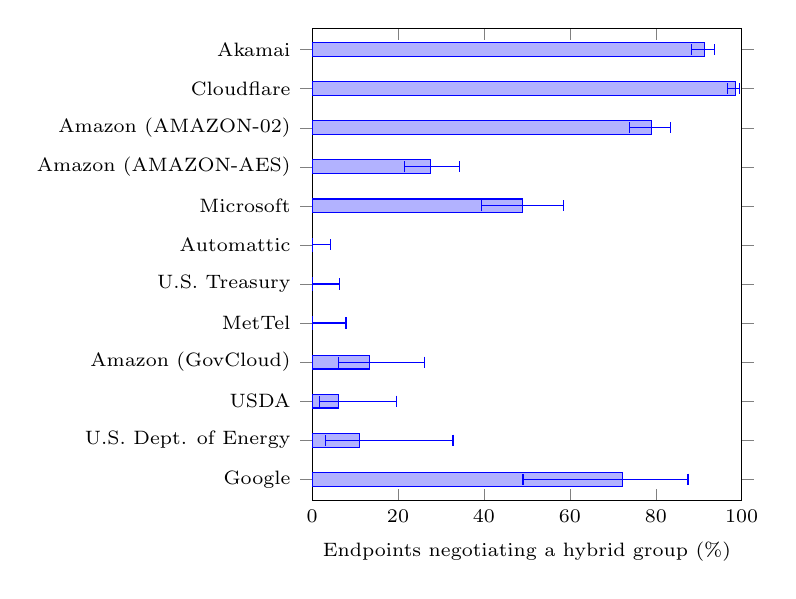
\begin{tikzpicture}
\begin{axis}[
  xbar, xmin=0, xmax=100, scale only axis, width=0.45\linewidth, height=6cm,
  xlabel={Endpoints negotiating a hybrid group (\%)},
  ytick={0,...,11},
  yticklabels={{Google},{U.S. Dept. of Energy},{USDA},{Amazon (GovCloud)},{MetTel},{U.S. Treasury},{Automattic},{Microsoft},{Amazon (AMAZON-AES)},{Amazon (AMAZON-02)},{Cloudflare},{Akamai}},
  y tick label style={font=\scriptsize}, x tick label style={font=\scriptsize},
  label style={font=\scriptsize}, bar width=5pt, enlarge y limits=0.05,
]
\addplot+[error bars/.cd, x dir=both, x explicit] coordinates {
  (72.2,0) += (15.3,0) -= (23.1,0)
  (11.1,1) += (21.7,0) -= (8.0,0)
  (6.1,2) += (13.5,0) -= (4.4,0)
  (13.3,3) += (12.8,0) -= (7.1,0)
  (0.0,4) += (7.9,0) -= (0.0,0)
  (0.0,5) += (6.3,0) -= (0.0,0)
  (0.0,6) += (4.3,0) -= (0.0,0)
  (49.0,7) += (9.6,0) -= (9.5,0)
  (27.5,8) += (6.8,0) -= (5.9,0)
  (79.1,9) += (4.4,0) -= (5.2,0)
  (98.6,10) += (0.8,0) -= (1.9,0)
  (91.4,11) += (2.3,0) -= (3.0,0)
};
\end{axis}
\end{tikzpicture}

\caption{Hybrid adoption among TLS endpoints in the
\data{rqtwo-asn-topk} autonomous systems hosting the most, with Wilson
95\% intervals.}
\label{fig:rq2-asn}
\end{figure}

\begin{table*}[t]
\centering\small
% Generated by paper/gen.py from paper/data. Do not edit.
\begin{tabular}{p{0.40\linewidth}rrrrrr}
\toprule
Autonomous system & TLS & Hyb. & Cl. & $\le$1.2 & Share & 95\% CI \\
\midrule
AS20940 Akamai International B.V. & 431 & 394 & 0 & 37 & 91.4\% & 88--94 \\
AS13335 Cloudflare, Inc. & 346 & 341 & 0 & 5 & 98.6\% & 97--99 \\
AS16509 Amazon (AMAZON-02) & 277 & 219 & 46 & 12 & 79.1\% & 74--83 \\
AS14618 Amazon (AMAZON-AES) & 189 & 52 & 110 & 27 & 27.5\% & 22--34 \\
AS8075 Microsoft Corporation & 102 & 50 & 26 & 26 & 49.0\% & 40--59 \\
AS2635 Automattic, Inc & 85 & 0 & 85 & 0 & 0.0\% & 0--4 \\
AS13506 U.S. Treasury & 57 & 0 & 6 & 51 & 0.0\% & 0--6 \\
AS16524 MetTel & 45 & 0 & 37 & 8 & 0.0\% & 0--8 \\
AS8987 Amazon (GovCloud) & 45 & 6 & 36 & 3 & 13.3\% & 6--26 \\
AS4155 USDA & 33 & 2 & 3 & 28 & 6.1\% & 2--20 \\
AS32982 U.S. Dept. of Energy & 18 & 2 & 5 & 11 & 11.1\% & 3--33 \\
AS396982 Google LLC & 18 & 13 & 5 & 0 & 72.2\% & 49--88 \\
\midrule
other 77 ASes & 314 & 51 & 130 & 133 & 16.2\% &  \\
\bottomrule
\end{tabular}

\caption{TLS endpoints by autonomous system: those that negotiated a hybrid
group (Hyb.), a classical TLS~1.3 group (Cl.) or no TLS~1.3 ($\le$1.2), for
the \data{rqtwo-asn-topk} ASes hosting the most, which hold
\data{rqtwo-asn-topk-cover} of TLS endpoints.}
\label{tab:rq2-asn}
\end{table*}

\paragraph{The provider decides.} Concurrent measurements of the wider web
found that managed infrastructure providers drive post-quantum
deployment~\cite{wickramasinghe2026} and that the provider predicts it
better than the organization's sector~\cite{loizou2026}. The federal web shows
the same pattern. Figure~\ref{fig:rq2-asn} and
Table~\ref{tab:rq2-asn} break adoption down by AS. Endpoints are
concentrated: the two largest ASes, Akamai and Cloudflare, hold
\data{rqtwo-top2-cover} of TLS endpoints and \data{rqtwo-top2-hybrid-cover}
of hybrid ones. Adoption there is \data{rqtwo-as20940-share} (Akamai) and
\data{rqtwo-as13335-share} (Cloudflare), and Fastly's
\data{rqtwo-as54113-n} endpoints are all hybrid. Large clouds sit in the
middle and differ by service: \data{rqtwo-as16509-share} on Amazon's main AS
but \data{rqtwo-as14618-share} on its AMAZON-AES AS and
\data{rqtwo-as8987-share} on GovCloud; \data{rqtwo-as8075-share} on Microsoft.
At the other end, none of the \data{rqtwo-as2635-n} endpoints hosted by
Automattic, the \data{rqtwo-as16524-n} on MetTel or the
\data{rqtwo-as13506-n} on the Treasury's own network negotiated a hybrid
group; on the Treasury's network \data{rqtwo-as13506-tlstwelve} of them do
not speak TLS~1.3.

What the federal population adds is the agency, the unit that M-26-15 holds
responsible for migration. To test whether the provider or the agency better
predicts the outcome, we
apply one rule to both groupings: among groups with at least
\data{rqtwo-uniform-min} TLS endpoints, what share of endpoints sit in a
group that is nearly uniform, with adoption at most \data{rqtwo-uniform-lo}
or at least \data{rqtwo-uniform-hi}? For ASes it is
\data{rqtwo-uniform-as-share} of endpoints (\data{rqtwo-uniform-as-groups}
ASes); for agencies, \data{rqtwo-uniform-agency-share}
(\data{rqtwo-uniform-agency-groups} agencies). Agencies are mixtures of
providers; providers are mostly all-or-nothing. Adoption among agencies with
at least \data{rqtwo-agency-min} TLS endpoints
(Table~\ref{tab:rq2-agencies} in the appendix) ranges from
\data{rqtwo-agency-min-share} to \data{rqtwo-agency-max}.

\paragraph{Certificates.} Post-quantum key exchange protects confidentiality
only; authentication is still classical everywhere. Of the
\data{rqtwo-cert-endpoints} TLS endpoints whose leaf certificate we recorded,
\data{rqtwo-cert-rsa-share} use RSA keys (\data{rqtwo-cert-rsa2048-share}
RSA-2048) and \data{rqtwo-cert-ecdsa-share} ECDSA keys; no other key type
appears.

\paragraph{Limits.} One vantage point and one moment: CDNs answer from the
edge nearest the scanner, and results may differ by location and over time.
The probe connects to the first resolved address, so a name served by two
providers is measured at one. A server that supports a hybrid group but
prefers X25519 when both are offered counts as classical, which is what a
browser would negotiate with it. We do not measure server software, which
would require an HTTP request beyond the handshake; the AS identifies the
hosting provider, not the software.

\section{RQ3: Quantum-Vulnerable Cryptography in Critical Open Source}
\label{sec:rq3}

\subsection{Method}

\paragraph{Projects.} The OpenSSF Criticality Score ranks open-source
projects by signals of how much depends on them~\cite{criticality}. We used its
latest published snapshot, \data{rqthree-snapshot}, pinned by commit and hash,
and walked down the top \data{rqthree-candidates} GitHub repositories. Many
top entries are copies of the same code base, mostly Linux kernel trees, so a
repository whose root commit matches a higher-ranked one was skipped as a
duplicate: \data{rqthree-duplicates} were, \data{rqthree-duplicates-kernel} of
them kernel trees. The first \data{rqthree-projects} distinct code bases, down
to rank \data{rqthree-last-rank}, are the sample. Repositories above
\data{rqthree-cap-gb}\,GB were counted but not cloned:
\data{rqthree-skipped-list}. One clone, \data{rqthree-failed-list}, failed
twice. That leaves \data{rqthree-scanned} scanned projects.

\paragraph{Scan.} Each project was cloned shallow at its default branch's head
and scanned with \tool{}'s source, configuration, dependency and binary layers
and reconciliation, with a \data{rqthree-timeout-min}-minute limit that no scan
reached (median \data{rqthree-scan-median}). Nothing was built or run. A
finding counts when its asset is quantum-vulnerable and it was found by a
layer rather than derived; derived findings are reported separately. Each
finding's exposure class comes from the risk engine: \emph{test} for test and
example paths; otherwise \emph{network-facing} for configuration and
key-material findings and for calls into TLS or SSH APIs; and
\emph{internal} for the rest.

\subsection{Results}

\begin{table}[t]
\centering\footnotesize\setlength{\tabcolsep}{4pt}
% Generated by paper/gen.py from paper/data. Do not edit.
\begin{tabular}{lrrrr}
\toprule
Projects with a finding & $n$ & Share & 95\% CI & Findings \\
\midrule
Any layer & 50 & 51.5\% & 42--61 & 7,596 \\
Used (source, config, binary) & 48 & 49.5\% & 40--59 & 6,323 \\
\emph{By layer} &  &  &  &  \\
\quad source & 32 & 33.0\% & 24--43 & 671 \\
\quad config and keys & 41 & 42.3\% & 33--52 & 5,637 \\
\quad dependencies & 26 & 26.8\% & 19--36 & 1,273 \\
\quad binaries & 2 & 2.1\% & 1--7 & 15 \\
\emph{By exposure class} &  &  &  &  \\
\quad network-facing & 22 & 22.7\% & 15--32 & 1,596 \\
\quad internal & 34 & 35.0\% & 26--45 & 1,366 \\
\quad test and example & 41 & 42.3\% & 33--52 & 4,634 \\
\emph{Derived findings} &  &  &  &  \\
\quad binary without source & 2 & 2.1\% & 1--7 & 9 \\
\quad stale dependency & 7 & 7.2\% & 4--14 & 20 \\
\bottomrule
\end{tabular}

\caption{Scanned projects with at least one quantum-vulnerable finding
($n$ of \data{rqthree-scanned}), with Wilson 95\% intervals, and the number
of findings. ``Used'' excludes dependency findings, which show a capability,
not a use.}
\label{tab:rq3-summary}
\end{table}

\paragraph{Prevalence.} Table~\ref{tab:rq3-summary} summarizes the scan.
\data{rqthree-any-n} of \data{rqthree-scanned} projects
(\data{rqthree-any-share}, CI \data{rqthree-any-ci}) contain
quantum-vulnerable cryptography in some layer, and
\data{rqthree-used-n} (\data{rqthree-used-share}) in their own source,
configuration or binaries, not only in dependencies. Configuration and key
material is the most common layer (\data{rqthree-config-share}), ahead of
source code (\data{rqthree-source-share}) and dependencies
(\data{rqthree-deps-share}); vulnerable code in committed binaries is rare
(\data{rqthree-binary-share}).

\paragraph{Exposure.} \data{rqthree-network-n} projects
(\data{rqthree-network-share}, CI \data{rqthree-network-ci}) have
quantum-vulnerable cryptography in network-facing code or configuration.
Test and example code is more common: \data{rqthree-test-share} of projects
have quantum-vulnerable findings there.

\paragraph{Algorithms.} RSA is the most widespread algorithm, in
\data{rqthree-alg-rsa-share} of scanned projects, followed by ECDSA
(\data{rqthree-alg-ecdsa-share}) and EdDSA (\data{rqthree-alg-eddsa-share});
Table~\ref{tab:rq3-algorithms} in the appendix lists all.

\paragraph{Reconciliation.} \data{rqthree-derived-stale-n} projects pin a
library version too old to offer post-quantum algorithms, and
\data{rqthree-derived-bws-n} ship binaries with cryptography their source
scan does not show. The other two derived types did not occur.
Declared-PQC-deployed-classical needs a probed endpoint, and RQ3 probes none.

\paragraph{Counts are concentrated.} Findings are not a measure of
prevalence. Five projects (\data{rqthree-top5-list}) account for
\data{rqthree-top5-share} of all quantum-vulnerable findings,
\data{rqthree-top5-config-share} of them certificates, keys and
configuration. The median
project with any finding has \data{rqthree-median-findings}. We report
shares of projects for this reason.

\subsection{Ranking Findings for Migration}

A project with hundreds of findings needs an order to migrate them in, which
is what \tool{}'s risk score gives (\S\ref{sec:design}). Its four factors
(exposure, secrecy lifetime, quantum status and confidence) carry weights we
chose by judgment, so we ablate them on the RQ3 findings. Each factor in turn
is set to one for every finding, the findings are re-scored, and each
project's ranking is compared with the full score's. That covers the
\data{riskabl-findings} findings of the \data{riskabl-projects} projects with
at least two, and the \data{riskabl-pairs} pairs of findings within a
project that the full score orders.

\begin{table}[t]
\centering\footnotesize\setlength{\tabcolsep}{4pt}
% Generated by paper/gen.py from paper/data. Do not edit.
\begin{tabular}{lrrrr}
\toprule
Factor removed & Reversed & Tied & Top changed & Median $\tau_b$ \\
\midrule
exposure & 6.8\% & 9.3\% & 45 (62\%) & 0.786 \\
secrecy lifetime & 12.1\% & 1.4\% & 28 (39\%) & 0.897 \\
quantum status & 16.4\% & 4.4\% & 34 (47\%) & 0.593 \\
confidence & 0.8\% & 1.2\% & 19 (26\%) & 0.992 \\
\bottomrule
\end{tabular}

\caption{Risk-score ablation over the \data{riskabl-projects} RQ3 projects
with at least two findings. Reversed and tied: share of the pairs the full
score orders that the ablated score orders the other way or ties. Top set
changed: projects whose highest-risk findings differ. $\tau_b$: Kendall's
rank correlation with the full score, median over projects.}
\label{tab:risk-ablation}
\end{table}

Table~\ref{tab:risk-ablation} gives the results. Every factor changes the
ranking, in different ways. Quantum status shapes the overall order most:
without it \data{riskabl-quantum-status-reversed} of ordered pairs reverse
and the median $\tau_b$ falls to \data{riskabl-quantum-status-tau}, because
hashes and symmetric ciphers then rank with RSA and elliptic curves.
Exposure decides what comes first: without it the top-risk findings change in
\data{riskabl-exposure-top} of \data{riskabl-projects} projects
(\data{riskabl-exposure-top-share}), and \data{riskabl-exposure-tied} of
pairs become ties. Secrecy lifetime reverses
\data{riskabl-secrecy-lifetime-reversed} of pairs. Confidence matters least: \data{riskabl-confidence-reversed}
of pairs reverse and the median $\tau_b$ stays at
\data{riskabl-confidence-tau}. It still changes the top set in \data{riskabl-confidence-top} projects. The
pair counts are pooled, so projects with many findings weigh most; the
$\tau_b$ median and the top-set count weigh each project once. The ablation
shows that each factor matters to the order, not that its weights are right:
validating them would need migration priorities set by the projects
themselves.

\paragraph{Limits.} \tool{}'s rules match cryptographic APIs, libraries and
configuration. A project that implements an algorithm itself shows few
findings: the Linux kernel tree in the sample, \data{rqthree-kernel-repo},
has \data{rqthree-kernel-findings}. Source rules cover Go, Python, Java, C/C++
and JavaScript/TypeScript; \data{rqthree-uncovered} scanned projects have a
primary language outside them (\data{rqthree-uncovered-top} and
\data{rqthree-uncovered-others} others) and are scanned in
the other layers only. Among the \data{rqthree-covered} in covered languages,
\data{rqthree-covered-source-share} have vulnerable source findings. The
network-facing class is a path and API heuristic, not reachability: it misses
cryptography reached from a network handler through other calls and includes
TLS configuration that no deployment uses. Finally, one shallow commit per
project is scanned on a case-insensitive file system, which drops one path of
each pair differing only in case.

\section{RQ4: The Cost of Migration}
\label{sec:rq4}

\subsection{Method}

\paragraph{Primitives.} We timed key generation, encapsulation and
decapsulation (or signing and verification) for the classical and
post-quantum schemes in Table~\ref{tab:rq4-primitives}, using Go's standard
library and CIRCL~\cite{circl} (\data{rqfour-circl}). X25519 and P-256 are
measured in KEM roles: encapsulation is the responder's work (parse the peer
key, generate an ephemeral key, derive the secret) and decapsulation the
initiator's. The hybrid is composed from Go's ML-KEM and X25519 as
\texttt{crypto/tls} composes it. Every call is timed individually; we report
the median (p50) of at least \data{rqfour-prim-min-n} calls. Before timing,
each scheme must round-trip: a decapsulation must recover the secret and a
signature must verify. The machine is an \data{rqfour-cpu} with
\data{rqfour-mem-gb}\,GB of memory, running \data{rqfour-kernel} and
Go~\data{rqfour-go}.

\paragraph{Sizes.} Public keys, ciphertexts and signatures are measured from
each implementation's output and compared with two independent sources: the
knowledge base's sizes and OpenSSL~3.5's output for the same parameter set.

\paragraph{Handshakes.} A Go TLS~1.3 server with an ECDSA P-256 certificate
and session resumption off serves three clients: one offering only X25519,
one offering only X25519MLKEM768, and Go's default client, which sends key
shares for both. We record the ClientHello and ServerHello sizes from the
record headers, the bytes each side sends, and the time from an established
TCP connection to a usable TLS connection. On the host, each client makes
\data{rqfour-host-n} handshakes over loopback. In a Linux container
(\data{rqfour-docker-kernel}) we shape the loopback interface with
\texttt{netem} into \data{rqfour-profiles} profiles: plain loopback, an MTU
of \data{rqfour-mtu} bytes, added round-trip times of \data{rqfour-rtt-list}\,ms,
and \data{rqfour-loss-rtt}\,ms with \data{rqfour-loss-pct} packet loss.

\subsection{Results}

\begin{table}[t]
\centering\small
% Generated by paper/gen.py from paper/data. Do not edit.
\begin{tabular}{lrr}
\toprule
Algorithm & \emph{public key} & \emph{ciphertext} \\
\midrule
X25519 & 32 & 32 \\
ECDH-P256 & 65 & 65 \\
ML-KEM-512 & 800 & 768 \\
ML-KEM-768 & 1,184 & 1,088 \\
ML-KEM-1024 & 1,568 & 1,568 \\
X25519MLKEM768 & 1,216 & 1,120 \\
\midrule
 & \emph{public key} & \emph{signature} \\
\midrule
RSA-2048 & 256 & 256 \\
RSA-3072 & 384 & 384 \\
ECDSA-P256 & 65 & $\le$72 \\
ML-DSA-44 & 1,312 & 2,420 \\
ML-DSA-65 & 1,952 & 3,309 \\
ML-DSA-87 & 2,592 & 4,627 \\
SLH-DSA-128s & 32 & 7,856 \\
SLH-DSA-128f & 32 & 17,088 \\
\bottomrule
\end{tabular}

\caption{Sizes in bytes on the wire. For X25519 and P-256 the ciphertext is
the ephemeral public key. ECDSA signatures vary in length (DER); the maximum
is shown.}
\label{tab:rq4-sizes}
\end{table}

\paragraph{Bytes.} Table~\ref{tab:rq4-sizes} gives the sizes. The hybrid key
share is \data{rqfour-size-x25519mlkem768-pk} bytes against
\data{rqfour-size-x25519-pk} for X25519, and its ciphertext
\data{rqfour-size-x25519mlkem768-ct}. All \data{rqfour-sizes-rows} measured
sizes agree with the knowledge base and, where OpenSSL can produce them
(\data{rqfour-sizes-openssl}), with OpenSSL, except the variable-length ECDSA
signature, which is not compared. On the wire, the hybrid ClientHello is
\data{rqfour-ch-hybrid} bytes against \data{rqfour-ch-classical}
(\data{rqfour-ch-ratio}), and Go's default ClientHello, which carries both key
shares, \data{rqfour-ch-default}. Even the hybrid ClientHello fits in one TCP
segment at an MTU of \data{rqfour-mtu} (\data{rqfour-mss} bytes of payload).
The ServerHello grows from \data{rqfour-sh-classical} to
\data{rqfour-sh-hybrid} bytes. Altogether a hybrid handshake moves
\data{rqfour-handshake-bytes-extra} more bytes. Post-quantum signatures would
cost more: an ML-DSA-65 signature is \data{rqfour-size-ml-dsa-65-sig} bytes
against \data{rqfour-size-rsa-2048-sig} for RSA-2048, before counting the
public key in each certificate of the chain.

\begin{table}[t]
\centering\footnotesize\setlength{\tabcolsep}{4pt}
% Generated by paper/gen.py from paper/data. Do not edit.
\begin{tabular}{llrrr}
\toprule
Algorithm & Impl. & keygen & encap & decap \\
\midrule
X25519 & Go & 35.2\,\textmu s & 70.0\,\textmu s & 34.8\,\textmu s \\
ECDH-P256 & Go & 11.1\,\textmu s & 52.0\,\textmu s & 40.8\,\textmu s \\
ML-KEM-512 & CIRCL & 21.8\,\textmu s & 23.6\,\textmu s & 21.0\,\textmu s \\
ML-KEM-768 & CIRCL & 37.0\,\textmu s & 39.2\,\textmu s & 28.8\,\textmu s \\
ML-KEM-1024 & CIRCL & 58.6\,\textmu s & 58.5\,\textmu s & 38.2\,\textmu s \\
ML-KEM-768 & Go & 35.5\,\textmu s & 36.7\,\textmu s & 38.9\,\textmu s \\
ML-KEM-1024 & Go & 54.5\,\textmu s & 59.4\,\textmu s & 63.2\,\textmu s \\
X25519MLKEM768 & Go & 70.7\,\textmu s & 107\,\textmu s & 73.8\,\textmu s \\
\midrule
 &  & keygen & sign & verify \\
\midrule
RSA-2048 & Go & 48.6\,ms & 929\,\textmu s & 28.8\,\textmu s \\
RSA-3072 & Go & 177\,ms & 2.60\,ms & 76.9\,\textmu s \\
ECDSA-P256 & Go & 11.6\,\textmu s & 21.8\,\textmu s & 54.8\,\textmu s \\
ML-DSA-44 & CIRCL & 80.2\,\textmu s & 147\,\textmu s & 73.3\,\textmu s \\
ML-DSA-65 & CIRCL & 145\,\textmu s & 238\,\textmu s & 120\,\textmu s \\
ML-DSA-87 & CIRCL & 216\,\textmu s & 259\,\textmu s & 199\,\textmu s \\
SLH-DSA-128s & CIRCL & 19.9\,ms & 151\,ms & 158\,\textmu s \\
SLH-DSA-128f & CIRCL & 311\,\textmu s & 7.30\,ms & 442\,\textmu s \\
\bottomrule
\end{tabular}

\caption{Median time per operation on the host (\data{rqfour-cpu}).
For signature schemes the columns are keygen, sign and verify.}
\label{tab:rq4-primitives}
\end{table}

\paragraph{Computation.} Table~\ref{tab:rq4-primitives} gives the operation
medians. Key exchange is cheap on both sides. Hybrid encapsulation takes
\data{rqfour-x25519mlkem768-go-stdlib-encap-p50}, \data{rqfour-hybrid-encap-vs-x25519}
X25519's, and a full hybrid exchange (keygen, encapsulation and
decapsulation) adds \data{rqfour-hybrid-kex-extra} of computation per
handshake. Signatures differ more. ML-DSA-65 signs in
\data{rqfour-ml-dsa-65-circl-sign-p50}, \data{rqfour-mldsa65-sign-vs-ecdsa}
ECDSA P-256 but RSA-2048 takes \data{rqfour-rsa2048-sign-vs-mldsa65} as long
as ML-DSA-65; ML-DSA-65 verification is
\data{rqfour-mldsa65-verify-vs-rsa2048} RSA-2048's. SLH-DSA-128s is the
outlier: \data{rqfour-slh-dsa-128s-circl-sign-p50} per signature,
\data{rqfour-slhs-sign-vs-mldsa65} ML-DSA-65.

\begin{table*}[t]
\centering\small
% Generated by paper/gen.py from paper/data. Do not edit.
\begin{tabular}{lrrrrrrrr}
\toprule
Profile & $n$ & \multicolumn{3}{c}{p50 handshake} & \multicolumn{2}{c}{Hybrid extra} & \multicolumn{2}{c}{p99} \\
\cmidrule(lr){3-5}\cmidrule(lr){6-7}\cmidrule(lr){8-9}
 &  & X25519 & Hybrid & Go def. & abs. & rel. & X25519 & Hybrid \\
\midrule
loopback & 200 & 0.31\,ms & 0.46\,ms & 0.45\,ms & 0.15\,ms & 48\% & 0.98\,ms & 1.48\,ms \\
loopback, MTU 1500 & 200 & 0.31\,ms & 0.46\,ms & 0.46\,ms & 0.15\,ms & 50\% & 0.60\,ms & 0.97\,ms \\
+2\,ms RTT & 200 & 4.74\,ms & 6.04\,ms & 5.92\,ms & 1.30\,ms & 28\% & 7.08\,ms & 7.86\,ms \\
+40\,ms RTT & 200 & 50.42\,ms & 51.77\,ms & 51.87\,ms & 1.35\,ms & 3\% & 61.15\,ms & 62.31\,ms \\
+40\,ms RTT, 1\% loss & 500 & 50.99\,ms & 51.17\,ms & 52.03\,ms & 0.18\,ms & 0\% & 320.28\,ms & 312.32\,ms \\
+150\,ms RTT & 200 & 163.44\,ms & 164.64\,ms & 164.61\,ms & 1.20\,ms & 1\% & 173.02\,ms & 173.51\,ms \\
\bottomrule
\end{tabular}

\caption{Full TLS~1.3 handshake time in the Linux container under each
\texttt{netem} profile, from established TCP connection to usable TLS
connection: medians for the X25519-only, hybrid-only and Go default
clients, the hybrid's extra median time over X25519, and p99.}
\label{tab:rq4-tls}
\end{table*}

\begin{figure}[t]
\centering
% Generated by paper/gen.py from paper/data. Do not edit.
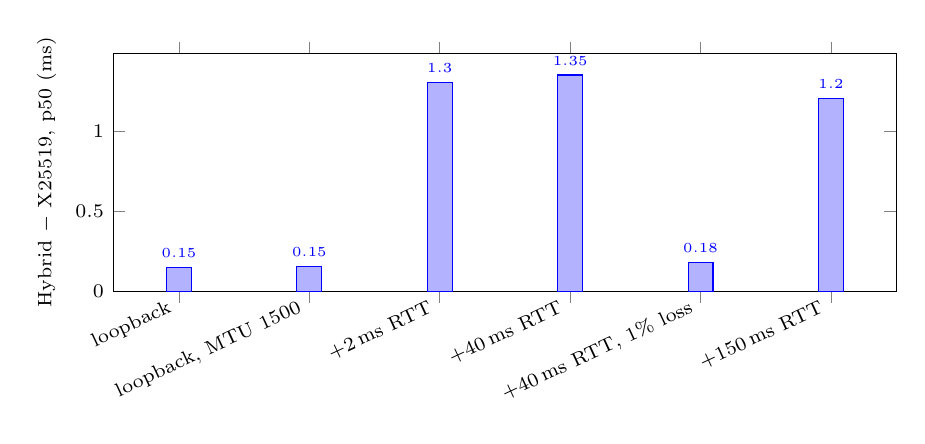
\begin{tikzpicture}
\begin{axis}[
  ybar, ymin=0, width=0.95\linewidth, height=4.6cm, bar width=9pt,
  symbolic x coords={{loopback},{loopback, MTU 1500},{+2\,ms RTT},{+40\,ms RTT},{+40\,ms RTT, 1\% loss},{+150\,ms RTT}}, xtick=data,
  x tick label style={font=\scriptsize, rotate=25, anchor=east},
  y tick label style={font=\scriptsize}, label style={font=\scriptsize},
  ylabel={Hybrid $-$ X25519, p50 (ms)},
  nodes near coords, every node near coord/.append style={font=\tiny, /pgf/number format/.cd, fixed, precision=2},
]
\addplot coordinates {({loopback},0.148) ({loopback, MTU 1500},0.154) ({+2\,ms RTT},1.303) ({+40\,ms RTT},1.349) ({+40\,ms RTT, 1\% loss},0.180) ({+150\,ms RTT},1.204)};
\end{axis}
\end{tikzpicture}

\caption{Extra median handshake time of X25519MLKEM768 over X25519, per
\texttt{netem} profile.}
\label{fig:rq4-extra}
\end{figure}

\paragraph{Latency.} Table~\ref{tab:rq4-tls} and Figure~\ref{fig:rq4-extra}
give the handshake results. On loopback the hybrid handshake's median is
\data{rqfour-loopback-extra} longer than the classical one
(\data{rqfour-loopback-extra-rel}), of the same order as the extra
computation (\data{rqfour-hybrid-kex-extra}). With
added delay the extra median is \data{rqfour-netem-extra-min} to
\data{rqfour-netem-extra-max}, and it does not grow with the round-trip time:
it is \data{rqfour-rtt150ms-extra} at \data{rqfour-rtt150ms-rtt}\,ms, or
\data{rqfour-rtt150ms-extra-rel} of the handshake. We have not isolated why
the extra time is larger with emulated delay than on plain loopback. Under
packet loss the tail is dominated by retransmissions for both clients.
None of the \data{rqfour-docker-handshakes} handshakes in the container
failed, and none of the host's.

\paragraph{Does cost explain non-adoption?} Our measurements suggest not.
At wide-area round-trip times the hybrid key exchange adds at most
\data{rqfour-netem-extra-max} at the median and
\data{rqfour-handshake-bytes-extra} bytes, and the hybrid ClientHello still
fits in a single segment. Go's default client already sends it, and RQ2 shows that
whether a federal endpoint negotiates it depends mostly on who hosts it.
Cost would matter more for post-quantum certificates: an ML-DSA-65 signature
is \data{rqfour-mldsa65-sig-vs-rsa2048} the size of an RSA-2048 one, and no
federal endpoint we measured uses one.
These results describe one machine and emulated links; middleboxes that
mishandle large ClientHellos are not represented.

\section{Discussion}
\label{sec:discussion}

\paragraph{Inventories need more than source code.} The federal migration
starts with discovery, and both M-26-15 and IR~8547 assume an inventory that
reflects what is deployed. RQ1 shows how much a source-only inventory misses
on a corpus that spreads assets across layers, and RQ3 shows the same pattern
in the field: configuration and key material is the layer where the most
critical projects most often carry quantum-vulnerable cryptography, and it
holds most of the findings. An inventory that reads only code misses that
layer entirely.

\paragraph{Hosting decides key exchange; authentication has not started.}
For key exchange the federal web is past half-way, but RQ2 suggests the
agencies did not get there one by one: endpoints behind Cloudflare, Akamai
and Fastly are nearly all hybrid, and endpoints on agency-run networks or on
some hosting platforms are nearly all classical. The quickest gains are
therefore at a handful of providers and at the \data{rqtwo-ep-tls1-2-or-lower}
endpoints that still lack TLS~1.3. Certificates are another matter. Every
leaf certificate we saw is RSA or ECDSA, and IR~8547's 2035 deadline applies
to signatures too. Their migration depends on post-quantum certificates being
issued and accepted, which no measured endpoint shows yet.

\paragraph{Threats to validity.} The RQ1 corpus was labeled by the author of
\tool{}'s rules; we release per-item outcomes and the competitors' raw output
so others can re-label. The risk score's weights are judgment calls, and this
draft does not yet ablate them. RQ2 is one vantage point at one moment, and
RQ3 one commit per project with a heuristic exposure model. RQ4 runs on one
machine with emulated links.

\paragraph{Future work.} Repeating the RQ2 scan monthly would turn the
snapshot into a trend. Data-flow analysis would recover the hard positives
\tool{} misses and give the exposure class real reachability. Probing the
endpoints that open-source projects deploy would let RQ3 measure the
declared-versus-deployed gap directly.

\section{Related Work}
\label{sec:related}

\paragraph{Finding cryptography in software.} Static analysis of
cryptographic code began with misuse: CryptoLint found that most Android apps
using cryptographic APIs misused them~\cite{egele2013}, and CrySL and
CryptoGuard check Java code against usage rules at scale~\cite{kruger2021crysl,
rahaman2019}, motivated in part by how hard developers find these
APIs~\cite{nadi2016}. These tools ask whether cryptography is used
correctly; an inventory asks what is used and where, including correct uses of
algorithms a quantum computer breaks. The open-source inventory tools we
compare in \S\ref{sec:rq1} (CBOMkit~\cite{cbomkit},
cryptoscan-pqc~\cite{cryptoscanpqc}, pqc-migration-audit~\cite{pqcaudit} and
Semgrep's rules~\cite{semgrep}) each cover one or two layers.
Olewinski et al.\ survey open-source cryptographic asset discovery tools and
find the landscape fragmented across categories~\cite{olewinski2026}; our
corpus measures that fragmentation as recall per layer. Other work covers
single layers in depth: Kestrel detects ML-KEM and ML-DSA implementations in
stripped binaries from their constant tables~\cite{junaid2026}, and Cho et al.\
flag quantum-vulnerable TLS from captured traffic~\cite{cho2026}. \tool{}'s
contribution is the combination: five layers normalized to one finding type
and reconciled, so that a gap between layers becomes a finding of its own.
For dependencies we follow the lesson of vulnerability analysis that a
library's presence is not its use~\cite{ponta2018}, and report dependency
findings as capabilities.

\paragraph{Post-quantum readiness of open source.} Yuan et al.\ measure
post-quantum support across eight package ecosystems and find it
rare~\cite{yuan2026}. RQ3 asks the converse question for the most critical
projects: how much quantum-vulnerable cryptography they carry, in which
layer, and how exposed it is. Library-level surveys track which libraries
offer the NIST algorithms~\cite{ahmed2025}, which is what \tool{}'s
dependency layer encodes.

\paragraph{Measurements of post-quantum handshakes.} Wickramasinghe et
al.~\cite{wickramasinghe2026} measure post-quantum TLS longitudinally across a
million domains from eleven vantage points, find that deployment centers on a
single hybrid construction driven by managed infrastructure providers, and see
no meaningful latency cost. Our results agree on all three. Dubey and
Varshney report hybrid key exchange on about half of a cross-sector domain list
and no post-quantum certificates~\cite{dubey2026}. Loizou and Ghadafi measure
UK organizations' HTTPS and mail endpoints and find, as we do, that the
provider predicts deployment better than the organization's
sector~\cite{loizou2026}. Haque et al.\ extend the measurement beyond HTTPS to
directory, mail and remote-access protocols, where support is lower,
mostly far lower~\cite{haque2026}. We differ in population and scope: the complete
registry of federal domains that EO~14412 and M-26-15 govern, broken down by
agency as well as provider, and paired with certificate and code-level
measurements. Singanamalla et al.\ measured the long tail of government adoption of
HTTPS itself~\cite{singanamalla2020}, and
certificate measurement at Internet scale goes back to
Durumeric et al.~\cite{durumeric2013https}.

\paragraph{Cost of post-quantum handshakes.} Paquin et al.\ benchmark post-quantum
key exchange and signatures in TLS under emulated network
conditions~\cite{paquin2020}, Sikeridis et al.\ study post-quantum
authentication in TLS~1.3~\cite{sikeridis2020}, and Kampanakis and
Childs-Klein measure the effect on time to last byte of real
connections~\cite{kampanakis2024}. The sizes of the NIST schemes follow from
their specifications~\cite{fips203,fips204,fips205}. RQ4 repeats the
measurement for the standardized hybrid group in a production TLS stack, the
one our probe is checked against, and cross-checks every size against OpenSSL.

\paragraph{Migration and crypto-agility.} A community workshop report frames
migration and crypto-agility as research problems~\cite{ott2019}. NIST's NCCoE migration project~\cite{nccoe} and CISA's
strategy for automated discovery and inventory tools~\cite{cisaacdi} make
discovery the starting point for federal agencies, which is the task \tool{}
automates.

\paragraph{Measurement ethics.} Our scanning practice follows the guidance
of the ZMap authors~\cite{zmap} and the Menlo Report~\cite{menlo}.

\section{Ethics}
\label{sec:ethics}

This work involves no human subjects. 
The RQ2 probes are the unauthenticated handshakes a browser starts. Each
endpoint received the probe's ClientHello and one standard handshake, each
retried a bounded number of times on failure, and no application data. The global rate was
\data{rqtwo-rate} connections per second and at most one connection per host
was open at a time, both enforced in code. Nothing was exploited and no
credentials were tried. The project's documentation describes exactly what a
probe sends and how to opt out; the opt-out list is honoured by every run and
held \data{rqtwo-exclude} entries at the time of the scan. We report results
in aggregate and will report notable findings about federal systems through
CISA. The scanning source address has no reverse DNS record pointing to the
project, which we note as a shortcoming of this run. RQ3 clones public
repositories and runs none of their code. These practices follow the
recommendations of the ZMap authors~\cite{zmap} and the Menlo
Report~\cite{menlo}.

\section{Conclusion}

Finding quantum-vulnerable cryptography is the first step every migration
plan requires, and it cannot be done from source code alone. \tool{} scans
five layers and reconciles them. It finds \data{rqone-recall-ratio} as many
labeled assets as the best open-source alternative, and it shows a federal web
where \data{rqtwo-ep-share} of TLS endpoints already negotiate hybrid key
exchange, largely because of where they are hosted, while every leaf
certificate remains classical. \data{rqthree-any-share} of the most critical open-source
code bases we scanned carry quantum-vulnerable cryptography, most often in configuration and key
material. Hybrid key exchange costs a kilobyte-scale ClientHello and, at the
median, at most \data{rqfour-netem-extra-max} per handshake in our
measurements, so its cost is unlikely to explain where it is missing.

\paragraph{Availability.} \tool{}, the corpus, the harness, the measurement
scripts, the raw data and this paper's generator are open source at
\url{https://github.com/emmanueladutwum123/pqscope}.


\bibliographystyle{plainnat}
\bibliography{refs}

\appendix
% Appendices, shared by main.tex and imc.tex. IMC requires the Ethics, Open
% Science and Generative AI sections.
\section{Ethics}
\label{sec:ethics}

This work involves no human subjects. 
The RQ2 probes are the unauthenticated handshakes a browser starts. Each
endpoint received the probe's ClientHello and one standard handshake, each
retried a bounded number of times on failure, and no application data. The global rate was
\data{rqtwo-rate} connections per second and at most one connection per host
was open at a time, both enforced in code. Nothing was exploited and no
credentials were tried. The project's documentation describes exactly what a
probe sends and how to opt out; the opt-out list is honoured by every run and
held \data{rqtwo-exclude} entries at the time of the scan. We report results
in aggregate and will report notable findings about federal systems through
CISA. The scanning source address has no reverse DNS record pointing to the
project, which we note as a shortcoming of this run. RQ3 clones public
repositories and runs none of their code. These practices follow the
recommendations of the ZMap authors~\cite{zmap} and the Menlo
Report~\cite{menlo}.


\section{Open Science}

Every artifact behind this paper is public: \tool{}'s source under the
Apache~2.0 license, the labeled corpus and the evaluation harness with every
competitor pinned by image digest, the measurement and benchmark scripts, the
raw measurement data (every probe record of RQ2 and every finding of RQ3),
and this paper's generator, at \artifactlink. Every number, table and figure is generated from the files in
\texttt{paper/data} by \texttt{paper/gen.py}, and a check fails the build if
any digit is typed into the paper's sources. The data come from these runs:
\begin{itemize}
\item RQ1: \texttt{make eval}, with competitors pinned by image digest.
\item RQ2: \texttt{measure/rq2.sh}, at \tool{} revision
  \rev{\data{rqtwo-revision}}, CISA list commit
  \texttt{\data{rqtwo-dotgov-commit}}, on \data{rqtwo-date}.
\item RQ3: \texttt{measure/rq3.sh}, at revision
  \rev{\data{rqthree-revision}}, Criticality Score snapshot
  \data{rqthree-snapshot} from commit
  \texttt{\data{rqthree-criticality-commit}}.
\item RQ4: \texttt{make bench}, at revision \rev{\data{rqfour-revision}},
  on \data{rqfour-date}.
\item RQ5: \texttt{measure/\allowbreak fed\_link.py} and
  \texttt{measure/\allowbreak fed\_scan.py},
  on \data{fed-date}, with GitHub's government registry at commit
  \texttt{\data{fed-registry-commit}} and the RQ2 records as the deployed side.
\item Risk-score ablation: \texttt{make risk-ablation}, at revision
  \rev{\data{riskabl-revision}}, from the RQ3 findings.
\end{itemize}

\section{Generative AI}

\textbf{[To be completed by the author before submission: state which
generative AI tools were used in this work, for what (for example writing
code, analysis scripts, or drafting and editing text), and how their output
was checked.]}

\section{Emulated-Link Handshakes}
\label{app:netem}

Table~\ref{tab:rq4-tls} and Figure~\ref{fig:rq4-extra} give the handshake
timings under emulated delay and loss that \S\ref{sec:rq4} sets aside. The
links were emulated with \texttt{netem} on the loopback interface of a Linux
container running in a virtual machine on the host of
Table~\ref{tab:rq4-primitives}. The hybrid's extra median time does not scale
with the added round-trip time, and we have not found the cause, so these
numbers should not be read as wide-area costs.

\begin{table*}[t]
\centering\small
% Generated by paper/gen.py from paper/data. Do not edit.
\begin{tabular}{lrrrrrrrr}
\toprule
Profile & $n$ & \multicolumn{3}{c}{p50 handshake} & \multicolumn{2}{c}{Hybrid extra} & \multicolumn{2}{c}{p99} \\
\cmidrule(lr){3-5}\cmidrule(lr){6-7}\cmidrule(lr){8-9}
 &  & X25519 & Hybrid & Go def. & abs. & rel. & X25519 & Hybrid \\
\midrule
loopback & 200 & 0.31\,ms & 0.46\,ms & 0.45\,ms & 0.15\,ms & 48\% & 0.98\,ms & 1.48\,ms \\
loopback, MTU 1500 & 200 & 0.31\,ms & 0.46\,ms & 0.46\,ms & 0.15\,ms & 50\% & 0.60\,ms & 0.97\,ms \\
+2\,ms RTT & 200 & 4.74\,ms & 6.04\,ms & 5.92\,ms & 1.30\,ms & 28\% & 7.08\,ms & 7.86\,ms \\
+40\,ms RTT & 200 & 50.42\,ms & 51.77\,ms & 51.87\,ms & 1.35\,ms & 3\% & 61.15\,ms & 62.31\,ms \\
+40\,ms RTT, 1\% loss & 500 & 50.99\,ms & 51.17\,ms & 52.03\,ms & 0.18\,ms & 0\% & 320.28\,ms & 312.32\,ms \\
+150\,ms RTT & 200 & 163.44\,ms & 164.64\,ms & 164.61\,ms & 1.20\,ms & 1\% & 173.02\,ms & 173.51\,ms \\
\bottomrule
\end{tabular}

\caption{Full TLS~1.3 handshake time in the Linux container under each
\texttt{netem} profile, from established TCP connection to usable TLS
connection: medians for the X25519-only, hybrid-only and Go default
clients, the hybrid's extra median time over X25519, and p99.}
\label{tab:rq4-tls}
\end{table*}

\begin{figure}[t]
\centering
% Generated by paper/gen.py from paper/data. Do not edit.
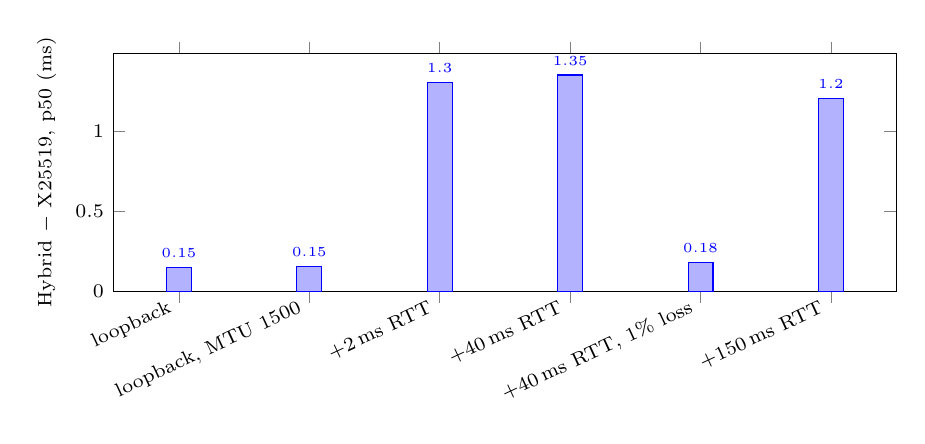
\begin{tikzpicture}
\begin{axis}[
  ybar, ymin=0, width=0.95\linewidth, height=4.6cm, bar width=9pt,
  symbolic x coords={{loopback},{loopback, MTU 1500},{+2\,ms RTT},{+40\,ms RTT},{+40\,ms RTT, 1\% loss},{+150\,ms RTT}}, xtick=data,
  x tick label style={font=\scriptsize, rotate=25, anchor=east},
  y tick label style={font=\scriptsize}, label style={font=\scriptsize},
  ylabel={Hybrid $-$ X25519, p50 (ms)},
  nodes near coords, every node near coord/.append style={font=\tiny, /pgf/number format/.cd, fixed, precision=2},
]
\addplot coordinates {({loopback},0.148) ({loopback, MTU 1500},0.154) ({+2\,ms RTT},1.303) ({+40\,ms RTT},1.349) ({+40\,ms RTT, 1\% loss},0.180) ({+150\,ms RTT},1.204)};
\end{axis}
\end{tikzpicture}

\caption{Extra median handshake time of X25519MLKEM768 over X25519, per
\texttt{netem} profile.}
\label{fig:rq4-extra}
\end{figure}

\clearpage
\section{Additional Tables}

\begin{table}[!htbp]
\centering\footnotesize\setlength{\tabcolsep}{4pt}
% Generated by paper/gen.py from paper/data. Do not edit.
\begin{tabular}{p{0.46\linewidth}rrrr}
\toprule
Agency & TLS & Hyb. & Share & 95\% CI \\
\midrule
Consumer Product Safety Commission & 20 & 20 & 100.0\% & 84--100 \\
Federal Trade Commission & 28 & 28 & 100.0\% & 88--100 \\
Library of Congress & 58 & 58 & 100.0\% & 94--100 \\
Department of Homeland Security & 74 & 70 & 94.6\% & 87--98 \\
Office of the Director of National Intelligence & 20 & 18 & 90.0\% & 70--97 \\
Department of Labor & 49 & 43 & 87.8\% & 76--94 \\
National Archives and Records Administration & 62 & 51 & 82.3\% & 71--90 \\
Department of Justice & 101 & 83 & 82.2\% & 74--88 \\
Department of Transportation & 26 & 21 & 80.8\% & 62--91 \\
Department of Commerce & 109 & 81 & 74.3\% & 65--82 \\
Government Publishing Office & 28 & 19 & 67.9\% & 49--82 \\
Department of the Interior & 97 & 65 & 67.0\% & 57--76 \\
Department of State & 28 & 18 & 64.3\% & 46--79 \\
Department of Defense & 45 & 23 & 51.1\% & 37--65 \\
United States House of Representatives & 38 & 19 & 50.0\% & 35--65 \\
Department of Health and Human Services & 196 & 97 & 49.5\% & 43--56 \\
Department of Education & 20 & 9 & 45.0\% & 26--66 \\
General Services Administration & 131 & 51 & 38.9\% & 31--47 \\
Executive Office of the President & 103 & 37 & 35.9\% & 27--46 \\
Department of the Treasury & 121 & 43 & 35.5\% & 28--44 \\
Department of Energy & 81 & 23 & 28.4\% & 20--39 \\
Office of Personnel Management & 29 & 6 & 20.7\% & 10--38 \\
Department of Agriculture & 51 & 10 & 19.6\% & 11--32 \\
\bottomrule
\end{tabular}

\caption{Hybrid adoption for agencies with at least \data{rqtwo-agency-min}
TLS endpoints, with Wilson 95\% intervals.}
\label{tab:rq2-agencies}
\end{table}

\begin{table}[!htbp]
\centering\small
% Generated by paper/gen.py from paper/data. Do not edit.
\begin{tabular}{lrrr}
\toprule
Algorithm & Projects & Share & Findings \\
\midrule
RSA & 49 & 51\% & 4,611 \\
ECDSA & 34 & 35\% & 1,878 \\
EdDSA & 29 & 30\% & 334 \\
X25519 & 25 & 26\% & 286 \\
ECDH & 24 & 25\% & 261 \\
DSA & 23 & 24\% & 151 \\
DH & 14 & 14\% & 33 \\
X448 & 14 & 14\% & 42 \\
\bottomrule
\end{tabular}

\caption{Quantum-vulnerable algorithms in the \data{rqthree-scanned} scanned
projects: projects with at least one finding, and findings.}
\label{tab:rq3-algorithms}
\end{table}


\end{document}
